\documentclass{beamer}

\mode<presentation> {
	\usetheme{CambridgeUS}%Boadilla
}
\usefonttheme[onlymath]{serif}
\usepackage{graphicx}
\usepackage{booktabs} % Allows the use of \toprule, \midrule and \bottomrule in tables
\usepackage{amsthm,amsmath,amssymb,mathrsfs}
\usepackage{amsfonts}
\usepackage{engord}
\usepackage{enumerate}
\usepackage{color}

%----------------------------------------------------------------------------------------

\title[ECMA, 2001]{Measuring Market Power in the Ready-to-Eat Cereal Industry}

\author{Aviv Nevo} 
\institute[]{Presenter: Qinzhu Sun}

\date{\today}
\logo{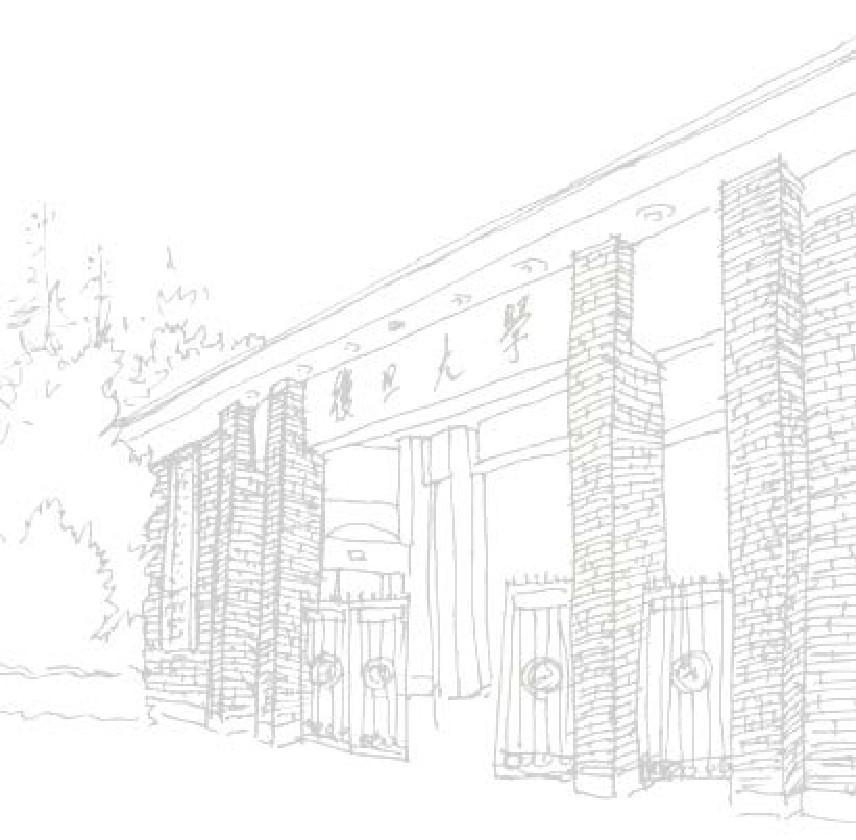
\includegraphics[scale=0.2]{maingate2}}
\begin{document}

\begin{frame}
\titlepage
\end{frame}
%------------------------------------------------

%------------------------------------------------
\section{Introduction}
\begin{frame}
	\transfade
	\tableofcontents[sectionstyle=show/shaded,subsectionstyle=show/shaded/hide]
	\addtocounter{framenumber}{-1}
\end{frame}
%------------------------------------------------
\begin{frame}[label=motivation]{Motivation}
	\begin{itemize}
		\item The ready-to-eat (RTE) cereal industry is characterized by
		\begin{itemize}
			\item high concentration
			\item high price-cost margins
			\item large advertising-to-sales ratios
			\item numerous introduction of new products
		\end{itemize}
		\item Previous researchers have concluded that the ready-to-eat cereal industry is a classic example of an industry with nearly collusive pricing behavior and intense nonprice competition.
	\end{itemize}
	\hyperlink{history}{\beamergotobutton{History of RTE}}
\end{frame}
%------------------------------------------------
\begin{frame}{This paper}
	\begin{itemize}
		\item This paper empirically examines this conclusion.
		\item In particular, this paper estimates price-cost margins and separates these margins into three sources
		\begin{itemize}
			\item product differentiation
			\item multi-product firm pricing
			\item price collusion
		\end{itemize}
		\item The results suggest that given the demand for different brands of cereal, the first two effects explain most of the observed price-cost margins.
		\begin{itemize}
			\item In particular, leading firms are able to maintain a portfolio of differentiated products and influence the perceived product quality. These two factors lead to high price-cost margins.
		\end{itemize}
	\end{itemize}
\end{frame}
%------------------------------------------------
\begin{frame}{General Strategy}
	\begin{itemize}
		\item Recall three sources of price-cost margins
		\begin{itemize}
			\item Product differentiation
			\item Portfolio effect
			\item Price collusion
		\end{itemize}
		\item General Strategy
		\begin{itemize}
			\item Estimate brand-level demand
			\item Then use the estimates jointly with pricing rules implied by different models of firm conduct to recover PCM
			\item Comparing the different sets of PCM to each other and to crude measure of actual PCM, allows me to separate the different sources of these margins.
		\end{itemize}
	\end{itemize}
\end{frame}
%------------------------------------------------
\begin{frame}{Difficulty}
	\begin{itemize}
		\item The data is three-dimensional panel of quantities and prices for 25 brands of cereal up to 65 U.S. cities over a period of 20 quarters.
		\item Two Challenges
		\begin{itemize}
			\item The correlation between prices and brand-city-quarter specific demand shocks (panel structure + IV)
			\item Large number of substitution parameters implied by numerous products in this industry (discrete choice model structure)
		\end{itemize}
	\end{itemize}
\end{frame}
%------------------------------------------------
\begin{frame}{Outline}
	\begin{itemize}
		\item Describe the ready-to-eat cereal industry
		\item Outline empirical model and discuss the implication of different modeling decisions
		\item Describe the data, the estimation procedure, instruments, and the inclusion of brand fixed effects
		\item Present the results
		\item Conclude
	\end{itemize}
\end{frame}
%------------------------------------------------

%------------------------------------------------
\section{The Ready-to-Eat Cereal Industry}
\begin{frame}
	\transfade
	\tableofcontents[sectionstyle=show/shaded,subsectionstyle=show/shaded/hide]
	\addtocounter{framenumber}{-1}
\end{frame}
%------------------------------------------------
\begin{frame}[label=history]{History}
	\begin{itemize}
		\item The first ready-to-eat breakfast cereal was probably introduced by James Caleb Jackson in 1863, in Dansville, New York.
		\item The real origin of the industry, however, was in Battle Creek, Michigan, where Dr. John Harvey Kellogg, the manager of vegetarian Seventh-Day Adventist (health) Sanatorium, introduced ready-to-eat cereal as a healthy breakfast alternative.
		\item Then later entrants include
		\begin{itemize}
			\item Post Cereal company
			\item Quaker Oats (General Mills)
			\item Nabisco
		\end{itemize}
	\end{itemize}
	\hyperlink{motivation}{\beamergotobutton{Motivation}}
\end{frame}
%------------------------------------------------
\begin{frame}{The Ready-to-Eat Cereal Industry}
	\begin{figure}[h]
		\centering
		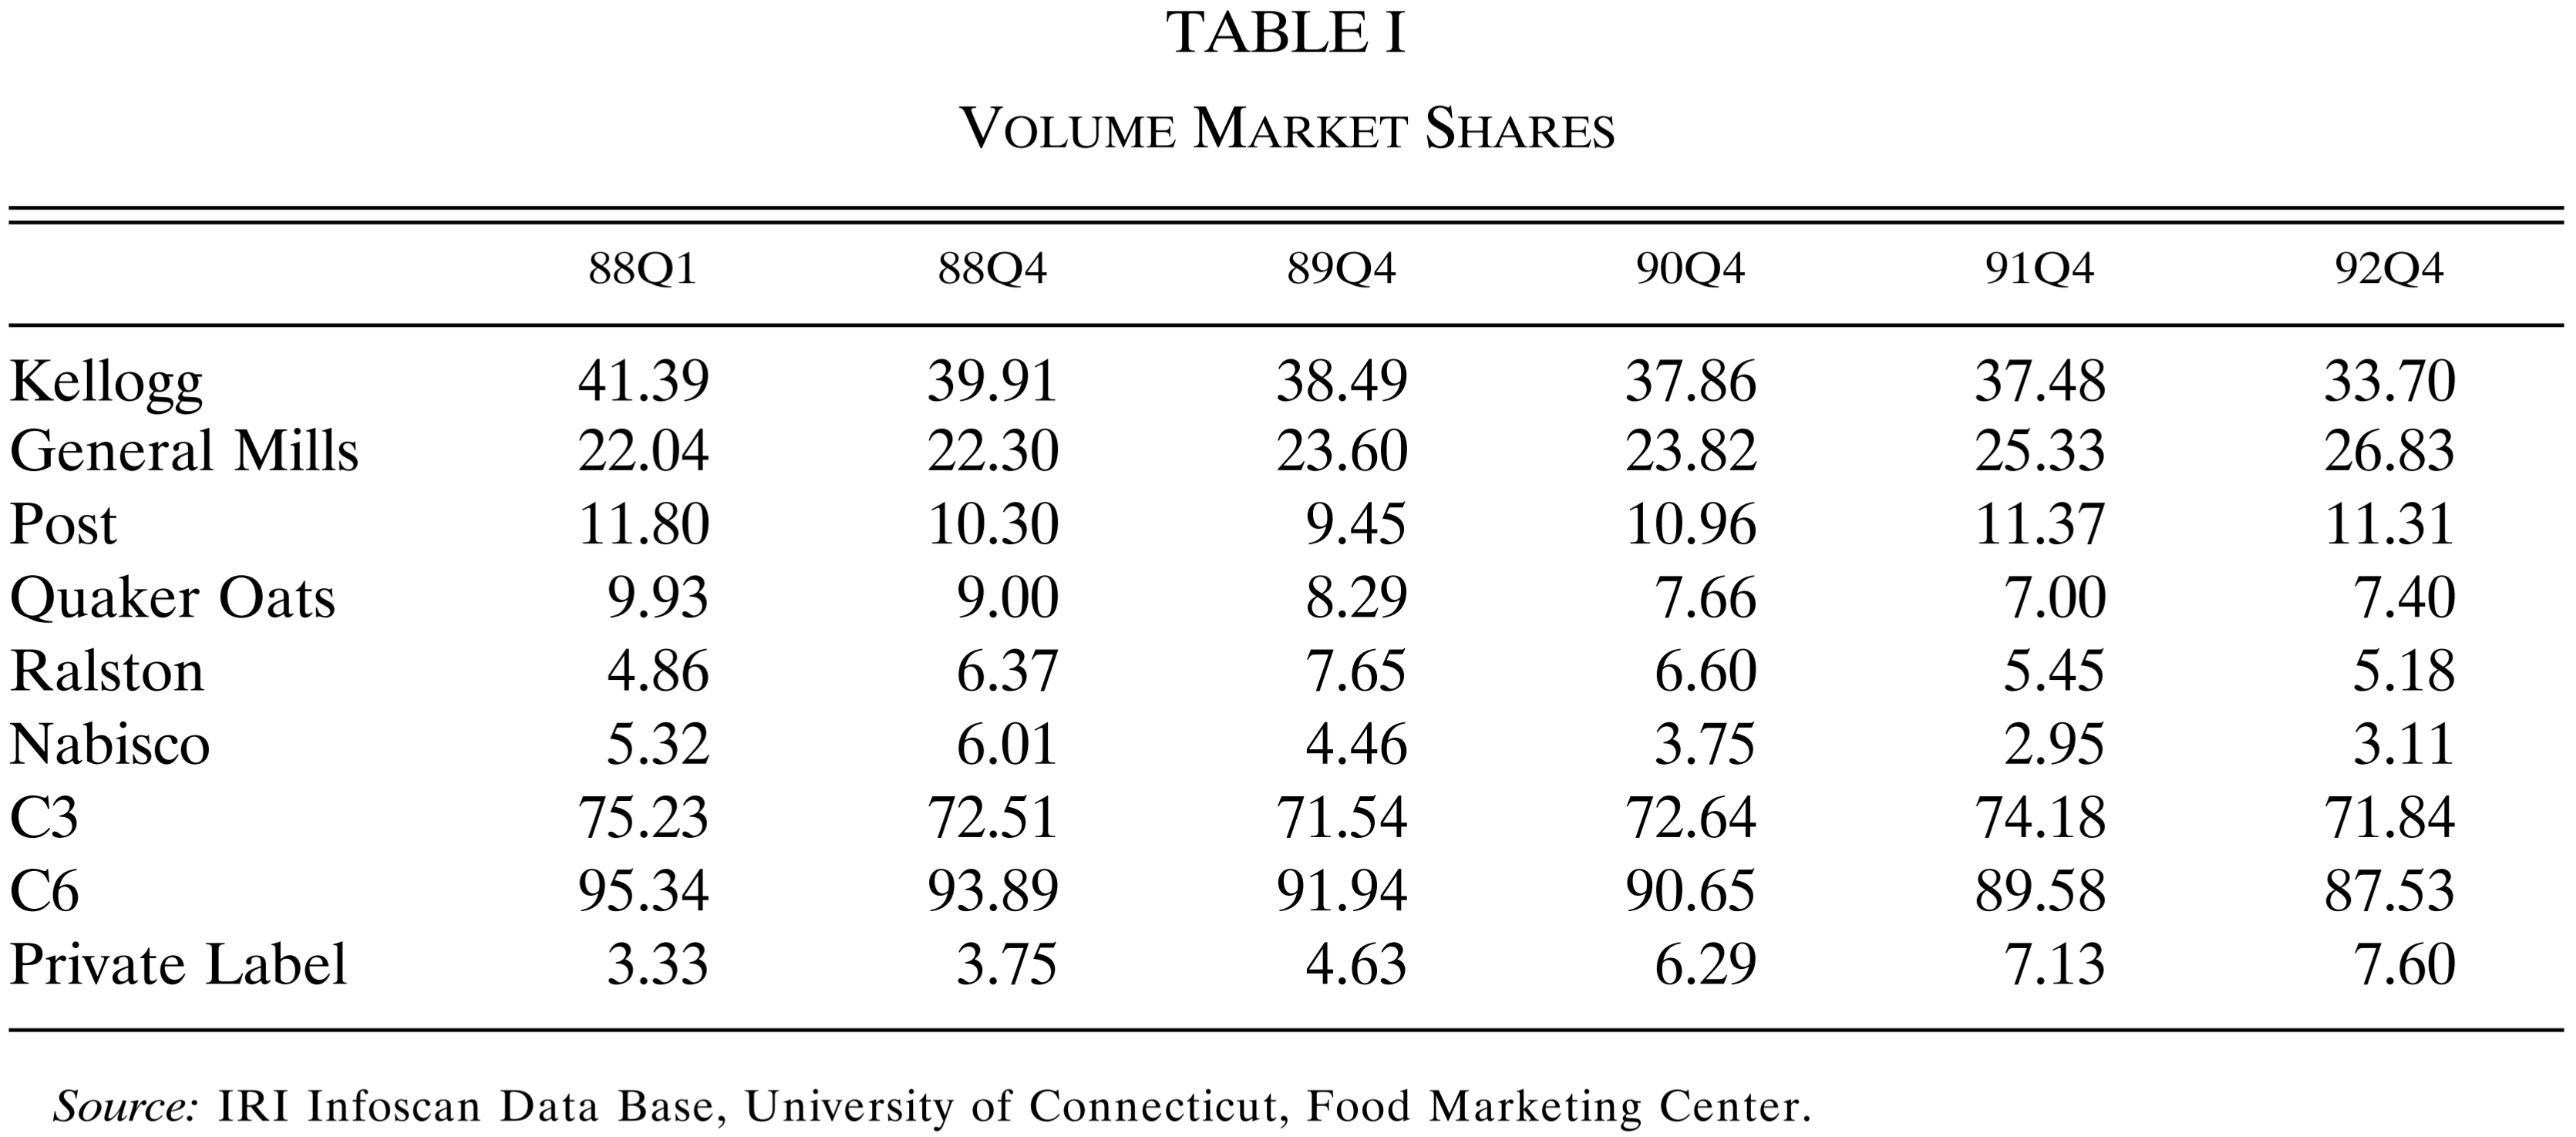
\includegraphics[scale=0.2]{table1.png}
	\end{figure}
\end{frame}
%------------------------------------------------
\begin{frame}{The Ready-to-Eat Cereal Industry}
	\begin{figure}[h]
		\centering
		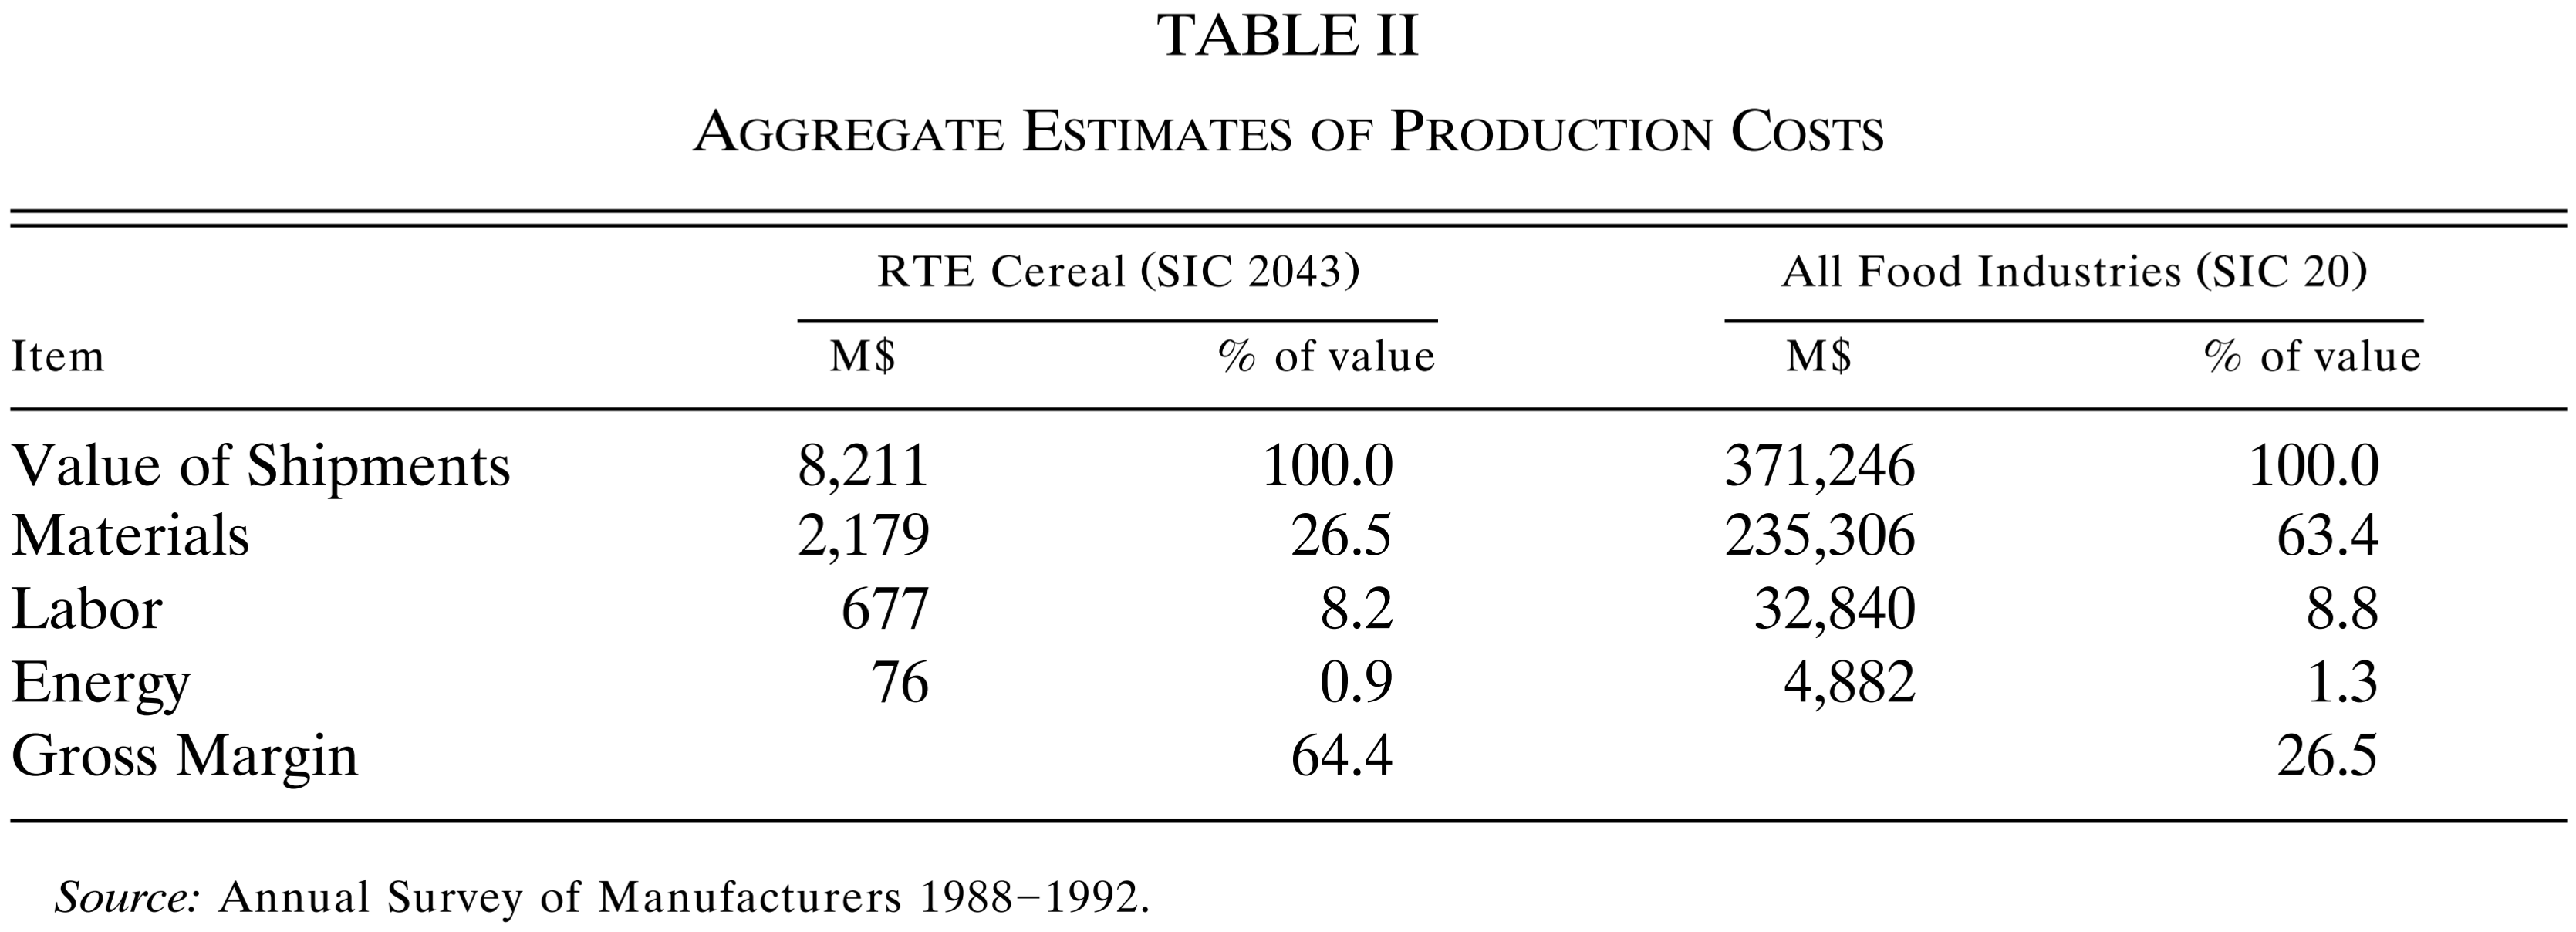
\includegraphics[scale=0.2]{table2.png}
	\end{figure}
\end{frame}
%------------------------------------------------

%------------------------------------------------
\section{The Empirical Framework}
\begin{frame}
	\transfade
	\tableofcontents[sectionstyle=show/shaded,subsectionstyle=show/shaded/hide]
	\addtocounter{framenumber}{-1}
\end{frame}
%------------------------------------------------
\begin{frame}{Outline}
	\begin{itemize}
		\item Consider different models of supply conduct
		\item For each model of supply, the pricing decision depends on brand-level demand, which is modeled as a function of product characteristics and consumer preferences.
		\item Demand parameters are estimated and used to compute the PCM implied by different models of conduct.
		\item Use additional information on costs to compute observed PCM and choose the conduct model that best fits these margins.
	\end{itemize}
\end{frame}
%------------------------------------------------

\begin{frame}{Supply}{Profit and FOC}
	\begin{itemize}
		\item Suppose there are $F$ firms, each of which produces some subset, $\mathscr{F}_f$, of the $j=1,...,J$ different brands of RTE cereal.
		\item The profits of firm $f$ are
		\begin{equation}\nonumber
			\Pi_f=\sum_{j\in\mathscr{F}_f}(p_j-mc_j)Ms_j(p)-C_f,
		\end{equation}
		where $s_j(p)$ is market share of brand $j$, $M$ is the market size, and $C_f$ is the fixed cost of production.
		\item Assuming the existence of pure-strategy Bertrand-Nash equilibrium in prices, the F.O.C. is:
		\begin{equation}\nonumber
			s_j(p)+\sum_{r\in\mathscr{F}_f}(p_r-mc_r)\frac{\partial s_r(p)}{\partial p_j}=0.
		\end{equation}
	\end{itemize}
\end{frame}
%------------------------------------------------
\begin{frame}{Supply}{Markup}
	Define $S_{jr}=-\partial s_r/\partial p_j,\; j,r=1,...,J$,
	\begin{equation}\nonumber
		\Omega^*_{jr}=\begin{cases}
			1,\quad \mbox{if }\exists f:\{r,j\}\subset \mathscr{F}_f \\
			0,\quad \mbox{otherwise},
		\end{cases}
	\end{equation}
	and $\Omega$ is a $J\times J$ matrix with $\Omega_{jr}=\Omega^*_{jr}*S_{jr}$. The F.O.C. becomes
	\begin{equation}\nonumber
		s(p)-\Omega(p-mc)=0.
	\end{equation}
	$\Rightarrow$
	\begin{equation}
		p-mc=\Omega^{-1}s(p).
	\end{equation}
\end{frame}
%------------------------------------------------
\begin{frame}{Supply}{Strategy}
	In order to distinguish between 3 different markup causes, estimate by defining the ownership $\mathscr{F}_f$, and ownership matrix $\Omega^*$, and evaluate the PCM in 3 hypothetical industry conduct models:
	\medskip

	\begin{itemize}
		\item \textbf{the single-product firms}, in which the price of each brand is set by a profit-maximizing agent that considers only that brand's profits.
		\item \textbf{the current structure}, where multi-product firms set the prices of all their products jointly.
		\item \textbf{the joint profit-maximization of all the brands}, which corresponds to monopoly or perfect price collusion.
	\end{itemize}
\end{frame}
%------------------------------------------------
\begin{frame}{Demand}{Indirect Utility}
	A market ($t=1,...,T$) is defined as a city-quarter combination. The conditional indirect utility of consumer $i$ from product $j$ at market $t$ is
	\begin{equation}
		u_{ijt}=x_j\beta_i^*-\alpha_i^*p_{jt}+\xi_j+\Delta\xi_{jt}+\epsilon_{ijt},
	\end{equation}

	\begin{itemize}
		\item $x_j$ is a K-dimensional vector of observable product characteristics
		\item $\xi_j$ is the national mean valuation of the unobserved product characteristics
		\item $\Delta\xi_{jt}$ is a city-quarter specific deviation from this mean
	\end{itemize}
	\medskip
	$\Rightarrow$ Finally, $(\alpha_i^*,\beta_i^*)$ are $K+1$ individual-specific coefficients.
\end{frame}
%------------------------------------------------
\begin{frame}{Demand}{Consumers' Heterogeneity}
	Let
	\begin{equation}
		\begin{pmatrix}
			\alpha_i^*\\ \beta_i^*
		\end{pmatrix}
		=
		\begin{pmatrix}
			\alpha \\ \beta
		\end{pmatrix}
		+\Pi D_i +\Sigma v_i,\quad v_i\sim N(0,I_{K+1}),
	\end{equation}
	\begin{itemize}
		\item $D_i$ is a $d\times 1$ vector of demographic variables
		\item $\Pi$ is a $(K+1)\times d$ matrix of coefficients that measure how the taste characteristics vary with demographics
		\item $\Sigma$ is a scaling matrix.
	\end{itemize}
\end{frame}
%------------------------------------------------
\begin{frame}{Demand}{Indirect Utility}
	Indirect utility for outside option
	\begin{equation}\nonumber
		u_{i0t}=\xi_0+\pi_0D_i+\sigma_0v_{i0}+\epsilon_{i0t}.
	\end{equation}
	
	Indirect utility for inside goods
	\begin{equation}
		\begin{split}
			u_{ijt}=\delta_{jt}(x_j,p_{jt},\xi_j,\Delta\xi_{jt};\theta_1)+\mu_{ijt}(x_j,p_{jt},v_i,D_i;\theta_2)+\epsilon_{ijt},\\
			\delta_{jt}=x_j\beta-\alpha p_{jt}+\xi_j+\Delta\xi_{jt},\qquad \mu_{ijt}=[p_{jt},x_j]'*(\Pi D_i+\Sigma v_i).
		\end{split}
	\end{equation}

	\begin{itemize}
		\item $\theta_1=(\alpha,\beta)$ contains the linear parameters
		\item $\theta_2=(\mbox{vec}(\Pi),\mbox{vec}(\Sigma))$ contains the nonlinear parameters.
	\end{itemize}
\end{frame}
%------------------------------------------------
\begin{frame}{Demand}{Market Share}
	The set of unobserved variables that lead to the choice of good $j$:
	\begin{equation}\nonumber
		A_{jt}(x,p_{\cdot t},\delta_{\cdot t};\theta_2)=\{(D_i,v_i,\epsilon_{it})|u_{ijt}\geq u_{ilt}\;\forall l=0,1,...,J \}
	\end{equation}

	\begin{itemize}
		\item $x$ are the characteristics of all brands
		\item $p_{\cdot t}=(p_{1t},...,p_{Jt})'$
		\item $\delta_{\cdot t}=(\delta_{1t},...,\delta_{Jt})'$
	\end{itemize}
	\begin{equation}
		\Rightarrow s_{jt}(x,p_{\cdot t},\delta_{\cdot t};\theta_2)=\int_{A_{jt}}dP^*(D,v,\varepsilon)=\int_{A_{jt}}dP^*(\varepsilon)dP^*(v)dP^*(D).
	\end{equation}
\end{frame}
%------------------------------------------------
\begin{frame}{Demand}{How to Solve}
	\begin{itemize}
		\item A simplifying assumption commonly made is that consumer heterogeneity enters the model only through the separable additive random shocks $\varepsilon_{ijt}$, and that $\varepsilon_{ijt}\overset{i.i.d.}{\sim} \mbox{Type I EV}$. $\Rightarrow$ logit model.
		\item Slightly less restrictive models, in which the i.i.d. assumption is replaced with a variance structure, are available (the Generalized Extreme Value model; McFadden (1978)). However, they derive substitution patterns from a priori segmentation.
		\item The full model nests all of these other models and has several advantages over them.
	\end{itemize}
	
\end{frame}
%------------------------------------------------

%------------------------------------------------
\section{Data and Estimation}
\begin{frame}
	\transfade
	\tableofcontents[sectionstyle=show/shaded,subsectionstyle=show/shaded/hide]
	\addtocounter{framenumber}{-1}
\end{frame}
%------------------------------------------------
\begin{frame}{Data}
	\begin{itemize}
		\item 65 different cities (the exact number increases over time)
		\item \engordnumber{1} quarter, 1988 – \engordnumber{4} quarter, 1992
		\item 25 brands
	\end{itemize}

	\begin{figure}[h]
		\centering
		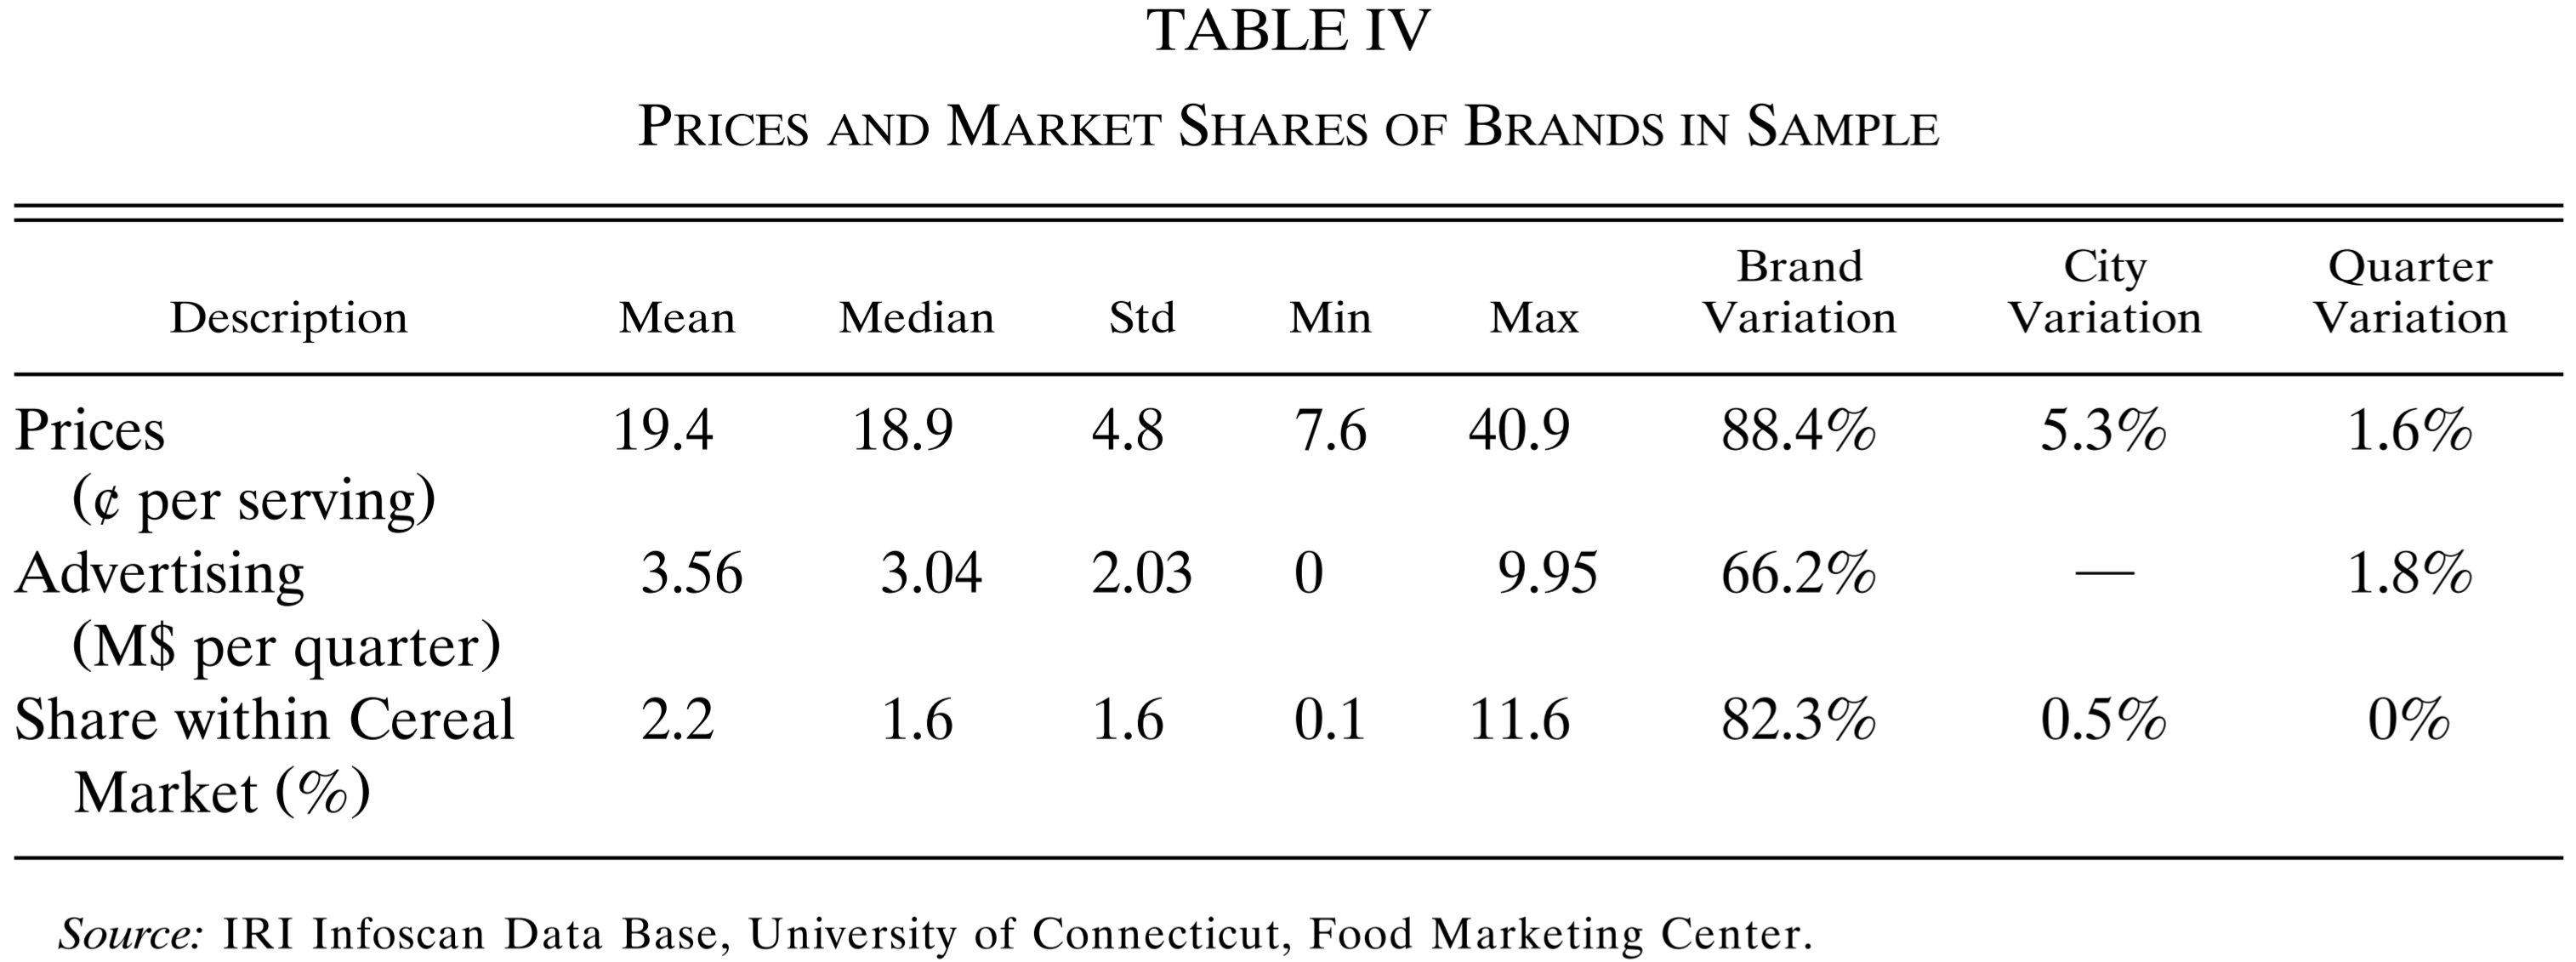
\includegraphics[scale=0.2]{table4.png}
	\end{figure}
\end{frame}
%------------------------------------------------
\begin{frame}{Comparison with BLP}
	Three key differences
	\begin{itemize}
		\item The instrumental variables and the identifying assumptions that support them are different.
		\medskip

		\item This paper identifies the demand side without specifying a functional form for the supply side.
		\medskip
	
		\item Due to data richness, this paper can control for unobserved product characteristics by using brand fixed effects.
	\end{itemize}
\end{frame}
%------------------------------------------------
\begin{frame}{GMM}
	Let $Z=[z_1,...,z_M]$ be a set of instruments such that $E[Z'\omega(\theta^*)=0]$.
	\begin{itemize}
		\item $\omega_{jt}=\xi_i+\Delta\xi_{jt}=\delta_{jt}(x,p_{\cdot t},\delta_{\cdot t};\theta_2)-(x_j\beta-\alpha p_{jt})$ is the unobserved product characteristics.
		\item $\theta^*$ denotes the true value of these parameters.
	\end{itemize}

	\begin{equation}
		\hat{\theta}=\underset{\theta}{\arg\min}\quad \omega(\theta)'ZA^{-1}Z'\omega(\theta),
	\end{equation}

	\begin{itemize}
		\item $A$ is a consistent estimate of $E[Z'\omega\omega'Z]$. $\Rightarrow$ two-step GMM.
	\end{itemize}
	\medskip

	Solve for the mean utility levels $\delta_{\cdot t}$
	\begin{equation}
		s_{\cdot t}(x,p_{\cdot t},\delta_{\cdot t};\theta_2)=S_{\cdot t} \quad\Rightarrow\quad \delta_{\cdot t}=\delta_{\cdot t}(x,p_{\cdot t},S_{\cdot t};\theta_2).
	\end{equation}
\end{frame}
%------------------------------------------------
\begin{frame}{Instruments}
	\begin{itemize}
		\item Pricing decision
		\begin{equation}
			p_{jt}=mc_{jt}+f(\xi_{jt},...)=(mc_j+f_j)+(\Delta mc_{jt}+\Delta f_{jt})
		\end{equation}
		\item Much of the previous work treats this endogeneity problem by assuming the “location” of brands in the characteristics space is exogenous, or at least predetermined.
		\item But by construction of the data, there is no variation in each brand’s observed characteristics over time and across cities.
		\item I use two alternative sets of IV
		\begin{itemize}
			\item price of the brand in other cities
			\item city-level marginal costs
		\end{itemize}
	\end{itemize}
\end{frame}
%------------------------------------------------
\begin{frame}{Instruments}
	\begin{itemize}
		\item The new strategy follows Hausman(1996) and exploits the panel structure of the data.
		\item The identifying assumption is that, controlling for brand-specific means and demographics, city-specific valuations are independent.
		\begin{itemize}
			\item Given this assumption, the prices of the brand in other cities will be valid IVs.
			\item The idea is prices of brand $j$ in two cities will be correlated due to the common marginal cost. According to the independent assumption across markets, prices will be uncorrelated with market specific valuation.
			\item This paper uses regional quarterly average prices in all twenty quarters.
		\end{itemize}
	\end{itemize}
\end{frame}
%------------------------------------------------
\begin{frame}{Potential Instrument Violation}
	Several plausible situations in which
	\begin{itemize}
		\item Case 1: suppose there is a national (or regional) demand shock. For example, the discovery that fiber reduces the risk of cancer. This discovery will increase the unobserved valuation of all fiber-intensive brands in all cities. (large companies)
		\item Case 2: suppose one believes that local advertising and promotions are coordinated across city borders, but are limited to regions, and that these activities influence demand. (large area)
	\end{itemize}
\end{frame}
%------------------------------------------------
\begin{frame}{Brand-Specific Dummy Variables}
	Why include brand-specific dummy variables as product characteristics
	\begin{itemize}
		\item improve the fit of the model
		\item captures the characteristics that do not vary by market. Therefore, the correlation between prices and the unobserved quality is fully accounted for and does not require IV.
	\end{itemize}

	Potential objections are defeated
	\begin{itemize}
		\item Introducing brand fixed effects increases the number of parameters only with $J$.
		\item Brand-specific intercepts enter as part of the linear parameters and do not increase the computational burden.
	\end{itemize}
\end{frame}
%------------------------------------------------
\begin{frame}[label=heterogeneity]{Brand-Specific Dummy Variables}
	In order to retrieve the taste coefficients $\beta$, when brand fixed-effects are included, I regress the estimated brand effects on the characteristics.

	Let
	$$d=X\beta+\xi.$$

	If we assume that $E[\xi|X]=0$, the estimates of $\beta$ and $\xi$ are
	$$\hat{\beta}=(X'V_d^{-1}X)^{-1}X'V_d^{-1}\hat{d},\qquad \hat{\xi}=\hat{d}-X\hat{\beta},$$
	where $\hat{d}$ is the vector of coefficients estimated from the procedure described previously, and $V_d$ is the covariance matrix of these estimates.
\end{frame}
%------------------------------------------------


%------------------------------------------------
\section{Results}
\begin{frame}
	\transfade
	\tableofcontents[sectionstyle=show/shaded,subsectionstyle=show/shaded/hide]
	\addtocounter{framenumber}{-1}
\end{frame}
%------------------------------------------------
\begin{frame}[label=logit]{Logit Results}
	Regress $\ln(X_{jt})-\ln(X_{0t})$ on prices, ad., brand and time dummy, to show
	\begin{itemize}
		\item importance of instrumenting for price
		\item effects of different sets of instrumental variables
	\end{itemize}

	\begin{figure}[h]
		\centering
		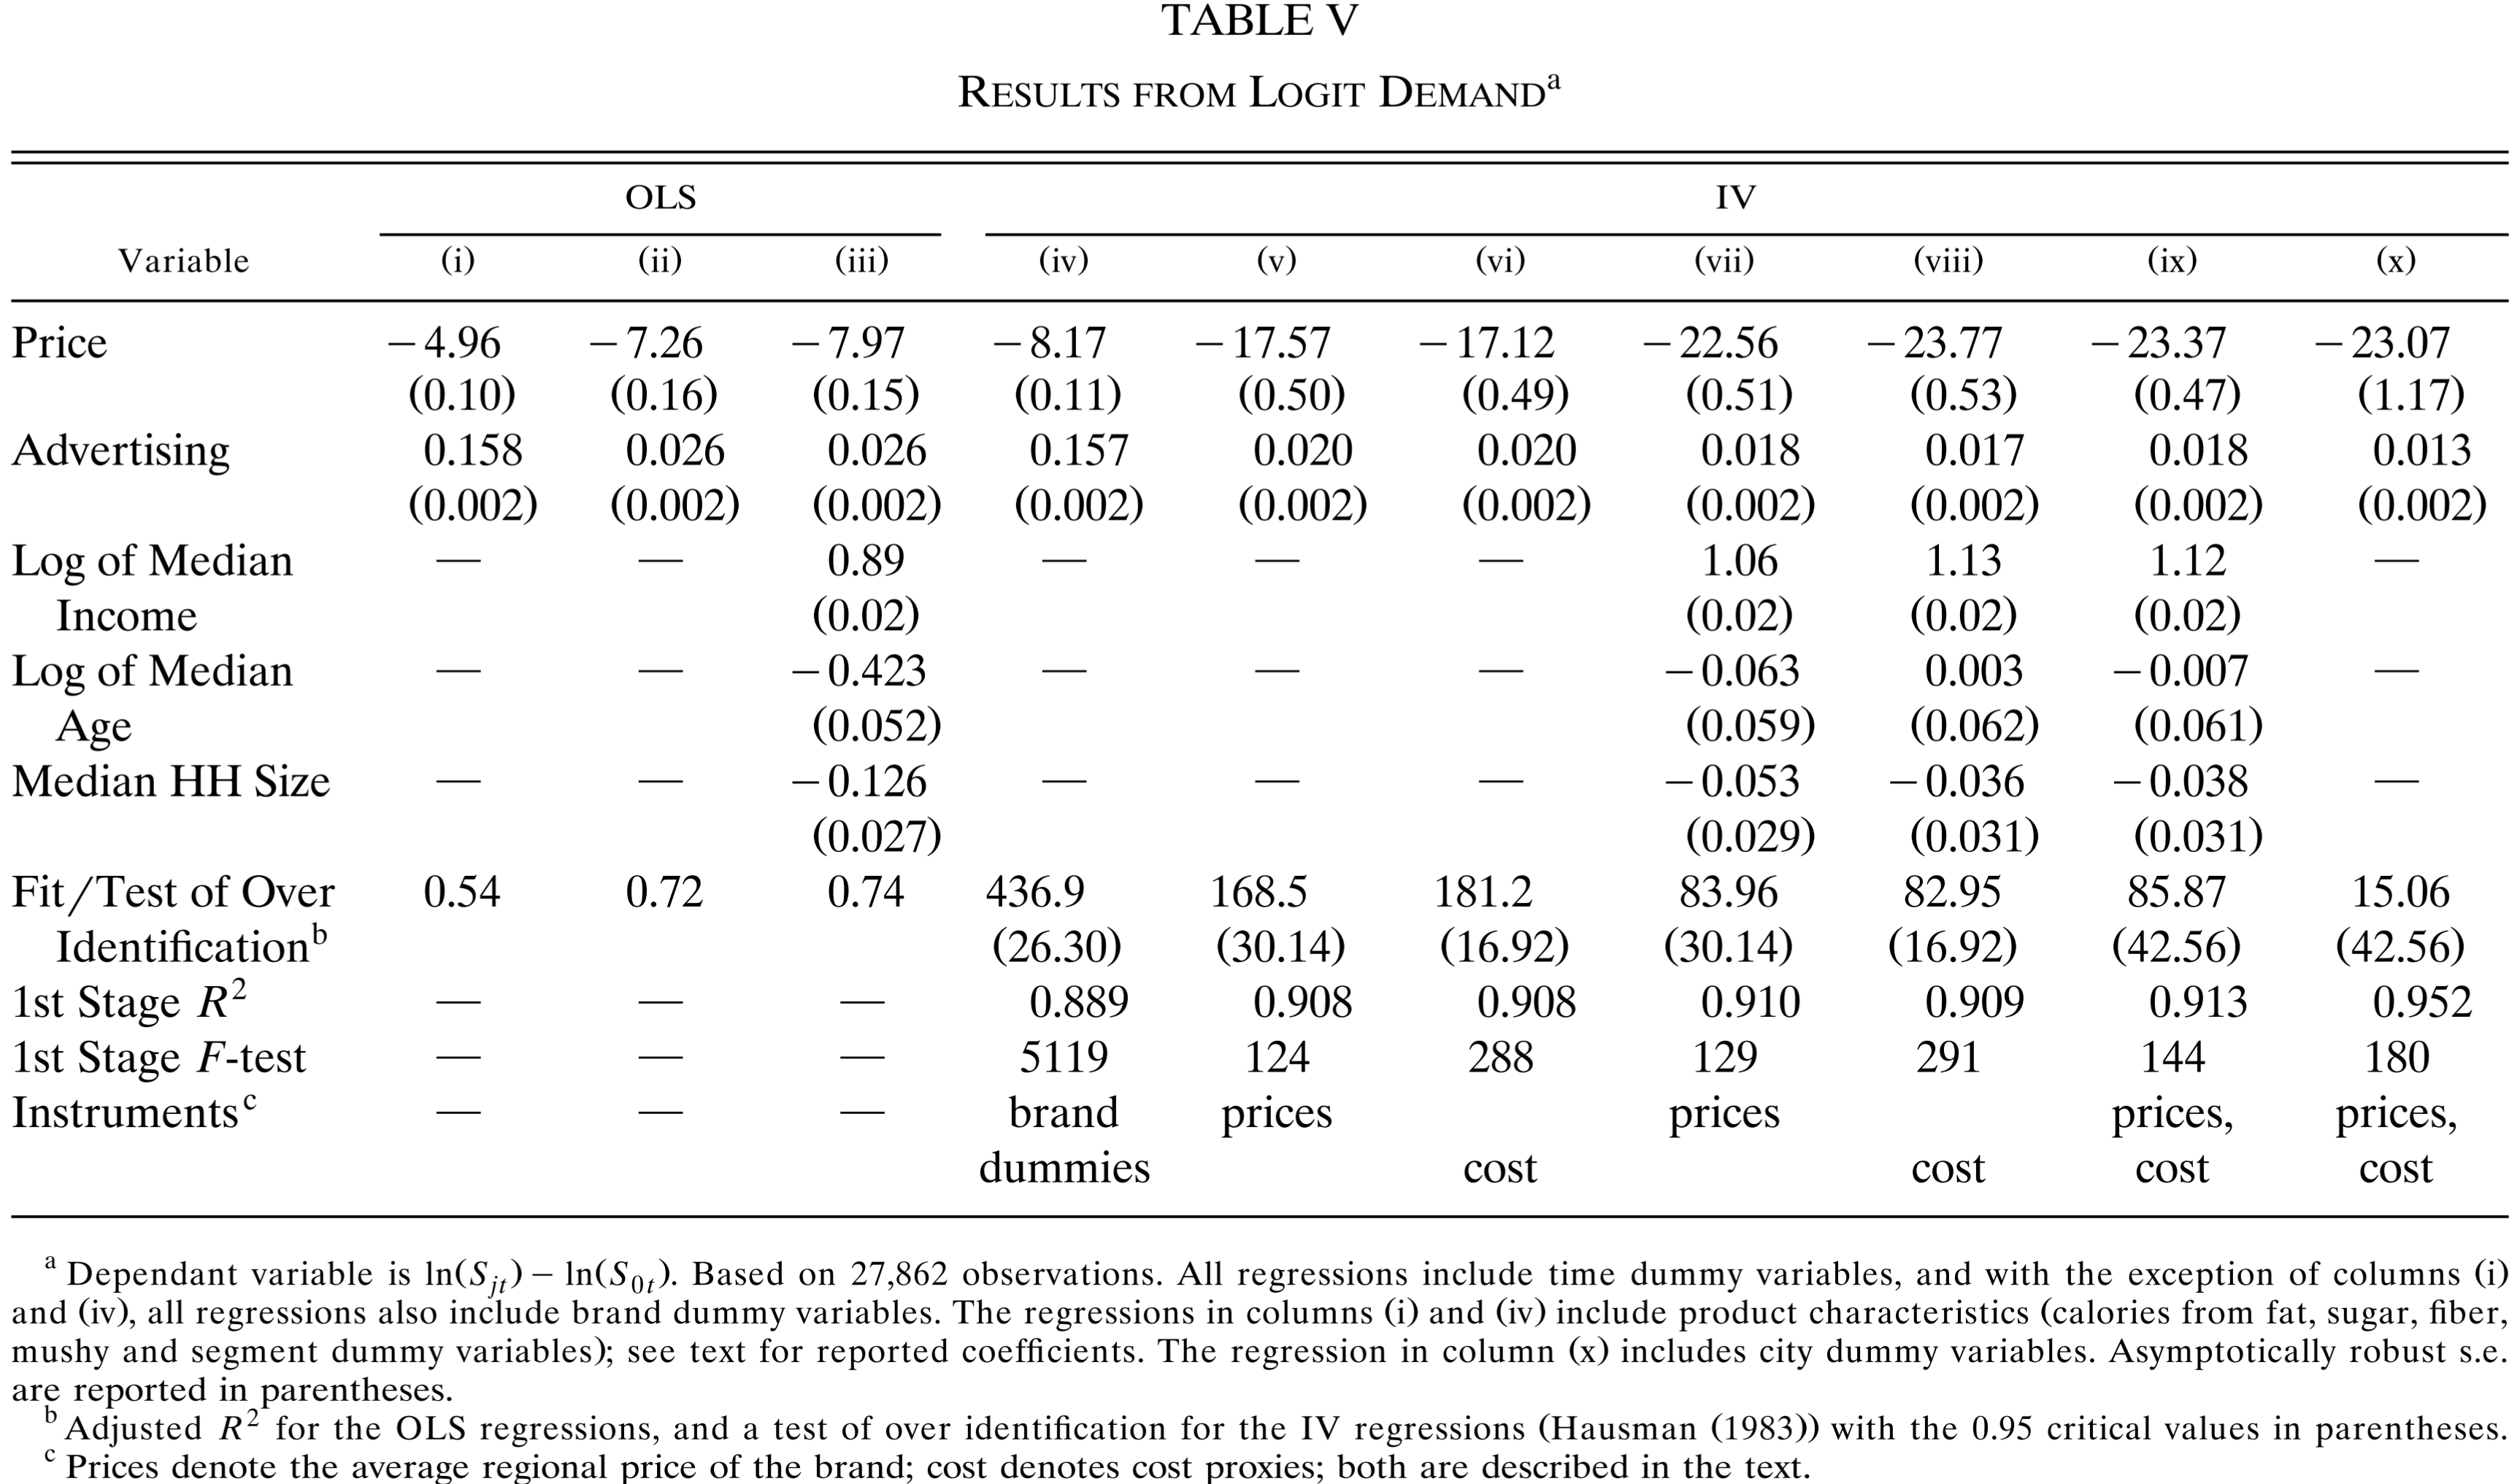
\includegraphics[scale=0.15]{table5.png}
	\end{figure}	
	\hyperlink{table8}{\beamergotobutton{Table 8 PCM}}
\end{frame}
%------------------------------------------------
\begin{frame}{Results from the Full Model}
	\begin{equation}\nonumber
		\begin{split}
			u_{ijt}=\delta_{jt}(x_j,p_{jt},\xi_j,\Delta\xi_{jt};\theta_1)+\mu_{ijt}(x_j,p_{jt},v_i,D_i;\theta_2)+\epsilon_{ijt},\\
			\delta_{jt}=x_j\beta-\alpha p_{jt}+\xi_j+\Delta\xi_{jt},\qquad \mu_{ijt}=[p_{jt},x_j]'*(\Pi D_i+\Sigma v_i).
		\end{split}
	\end{equation}
	\begin{itemize}
		\item Predicted market shares are based on the empirical distribution of 	demographics, independent normal distributions for $v$, and Type I extreme value for $\varepsilon$.
		\item The IV’s include both average regional prices in all quarters and the cost proxies.
	\end{itemize}	
\end{frame}
%------------------------------------------------
\begin{frame}[label=table6]{Results from the Full Model}
	The ratios of the variance explained by the demographics to the total variation in the distribution of the estimated coefficients: over 90\%.
	\begin{figure}[h]
		\centering
		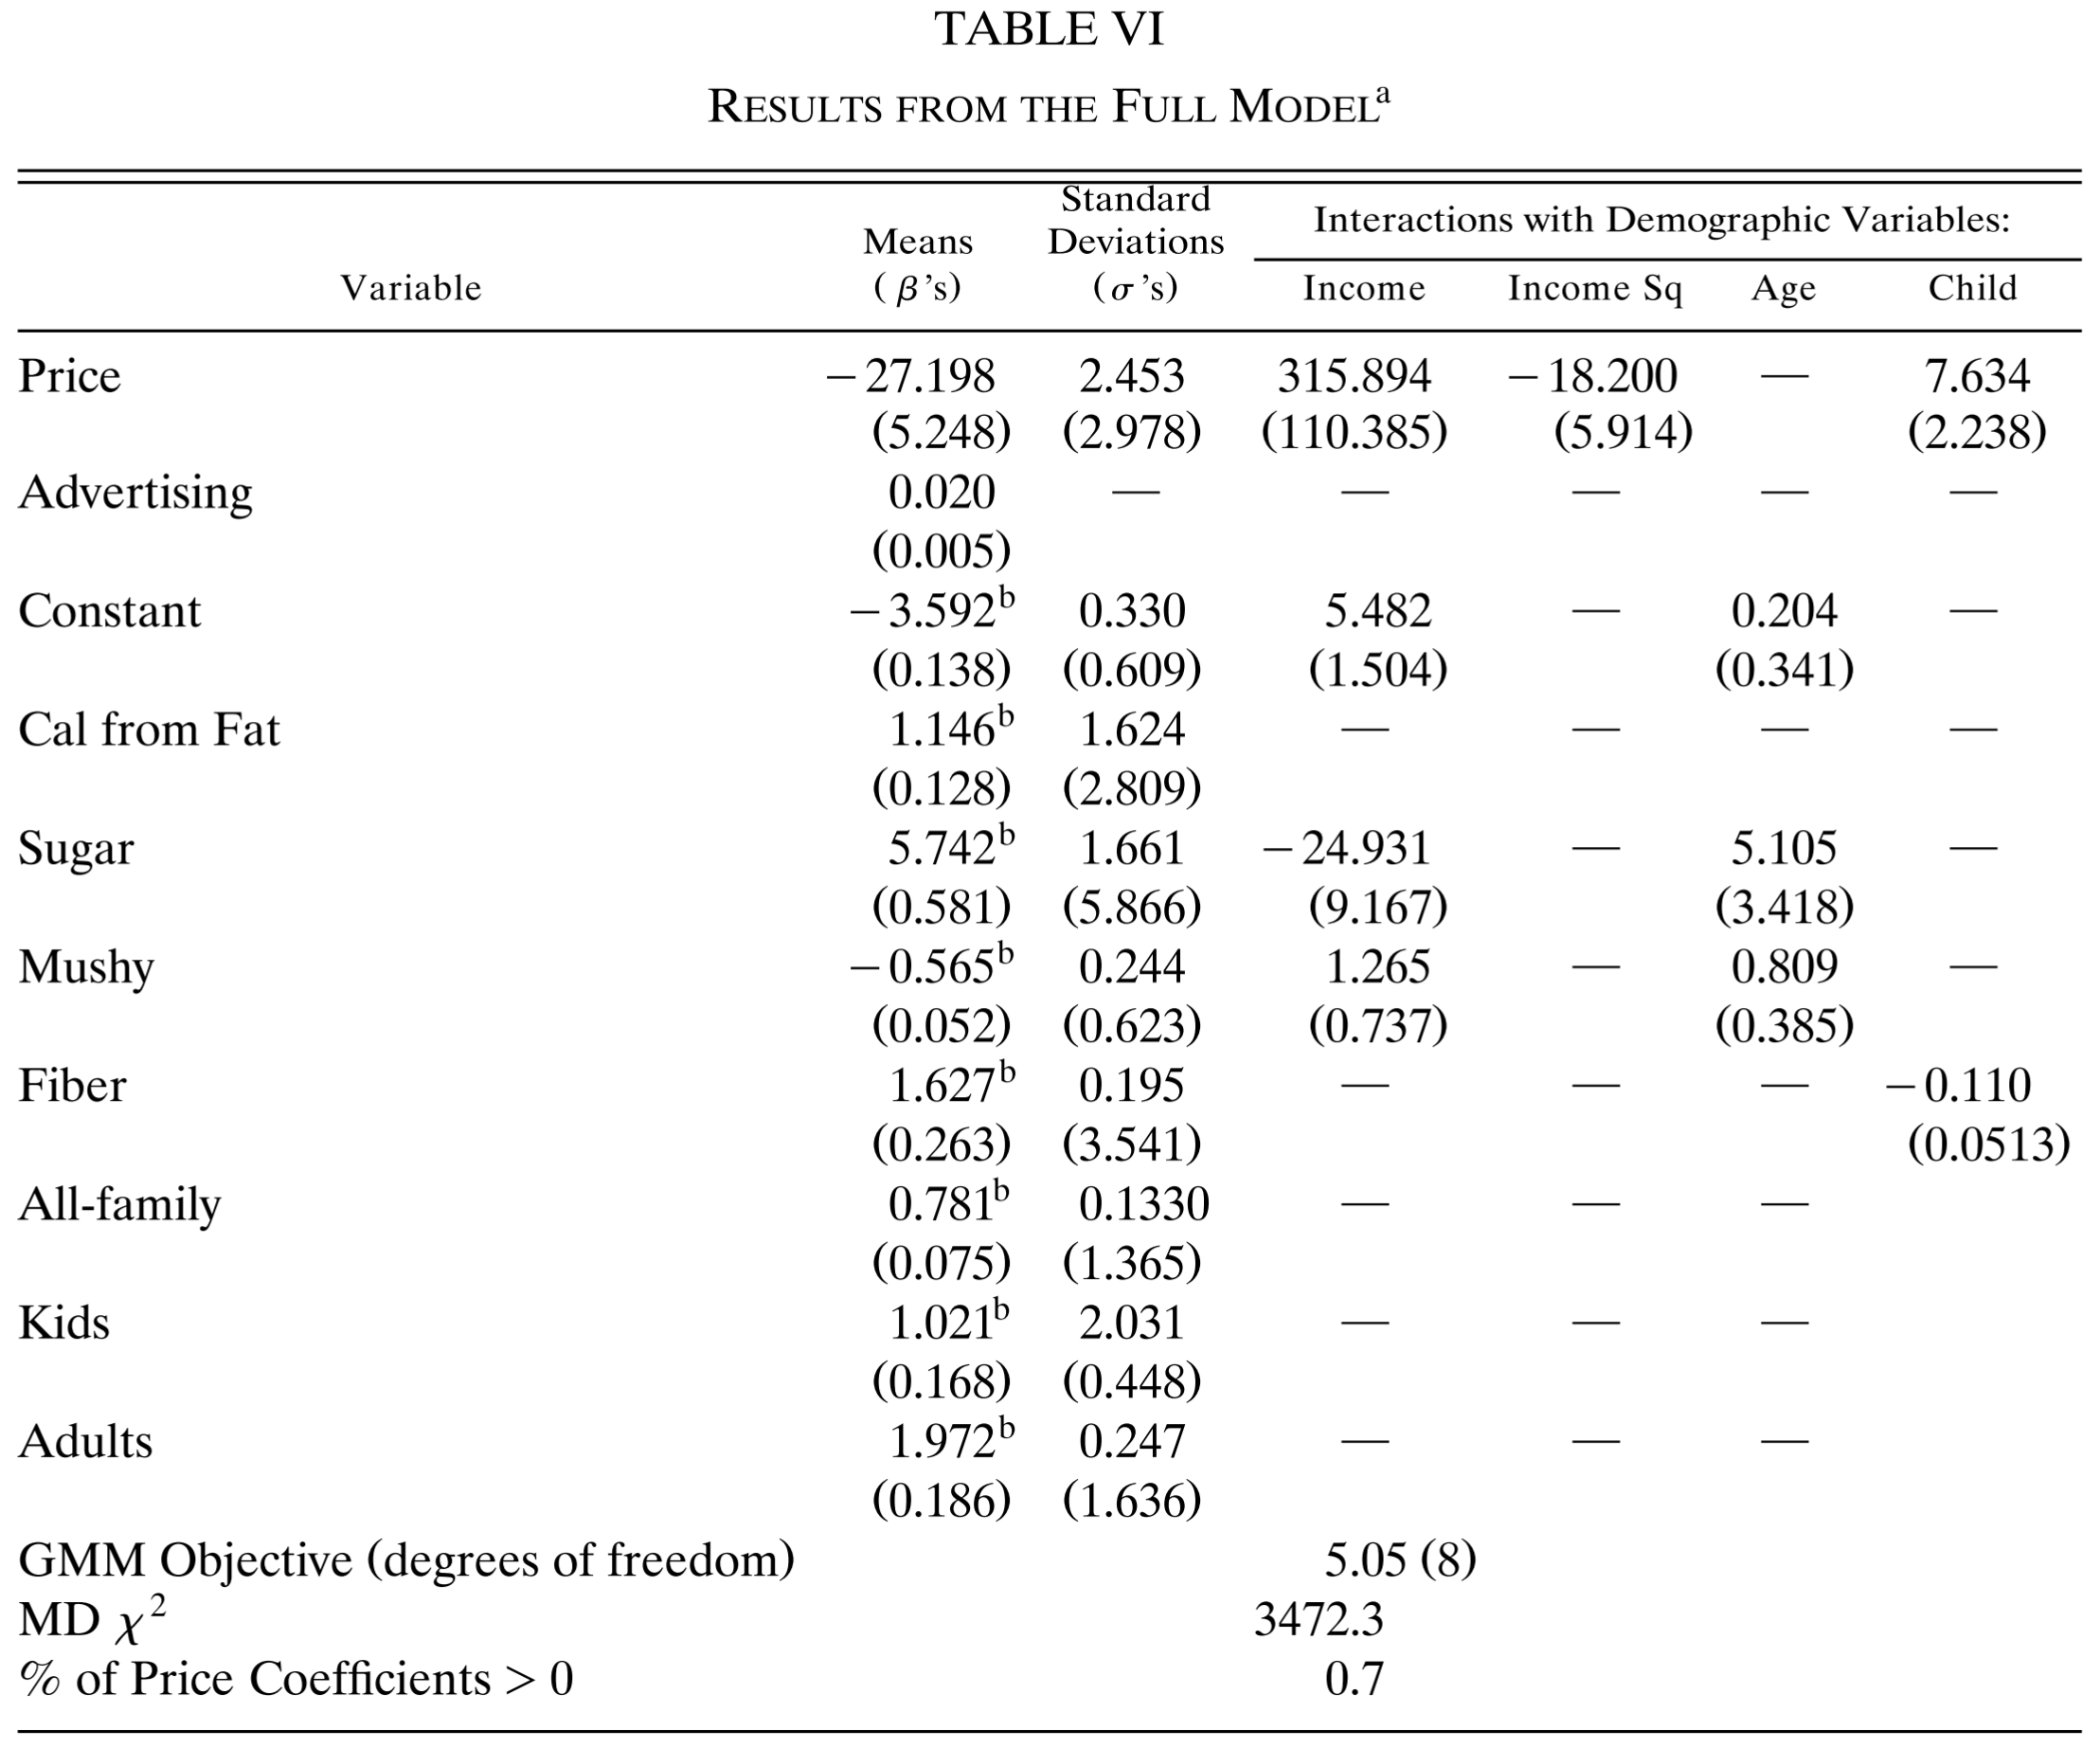
\includegraphics[scale=0.19]{table6.png}
	\end{figure}
\end{frame}
%------------------------------------------------
\begin{frame}{Taste Heterogeneity for Brand Characteristics}
	\begin{figure}[h]
		\centering
		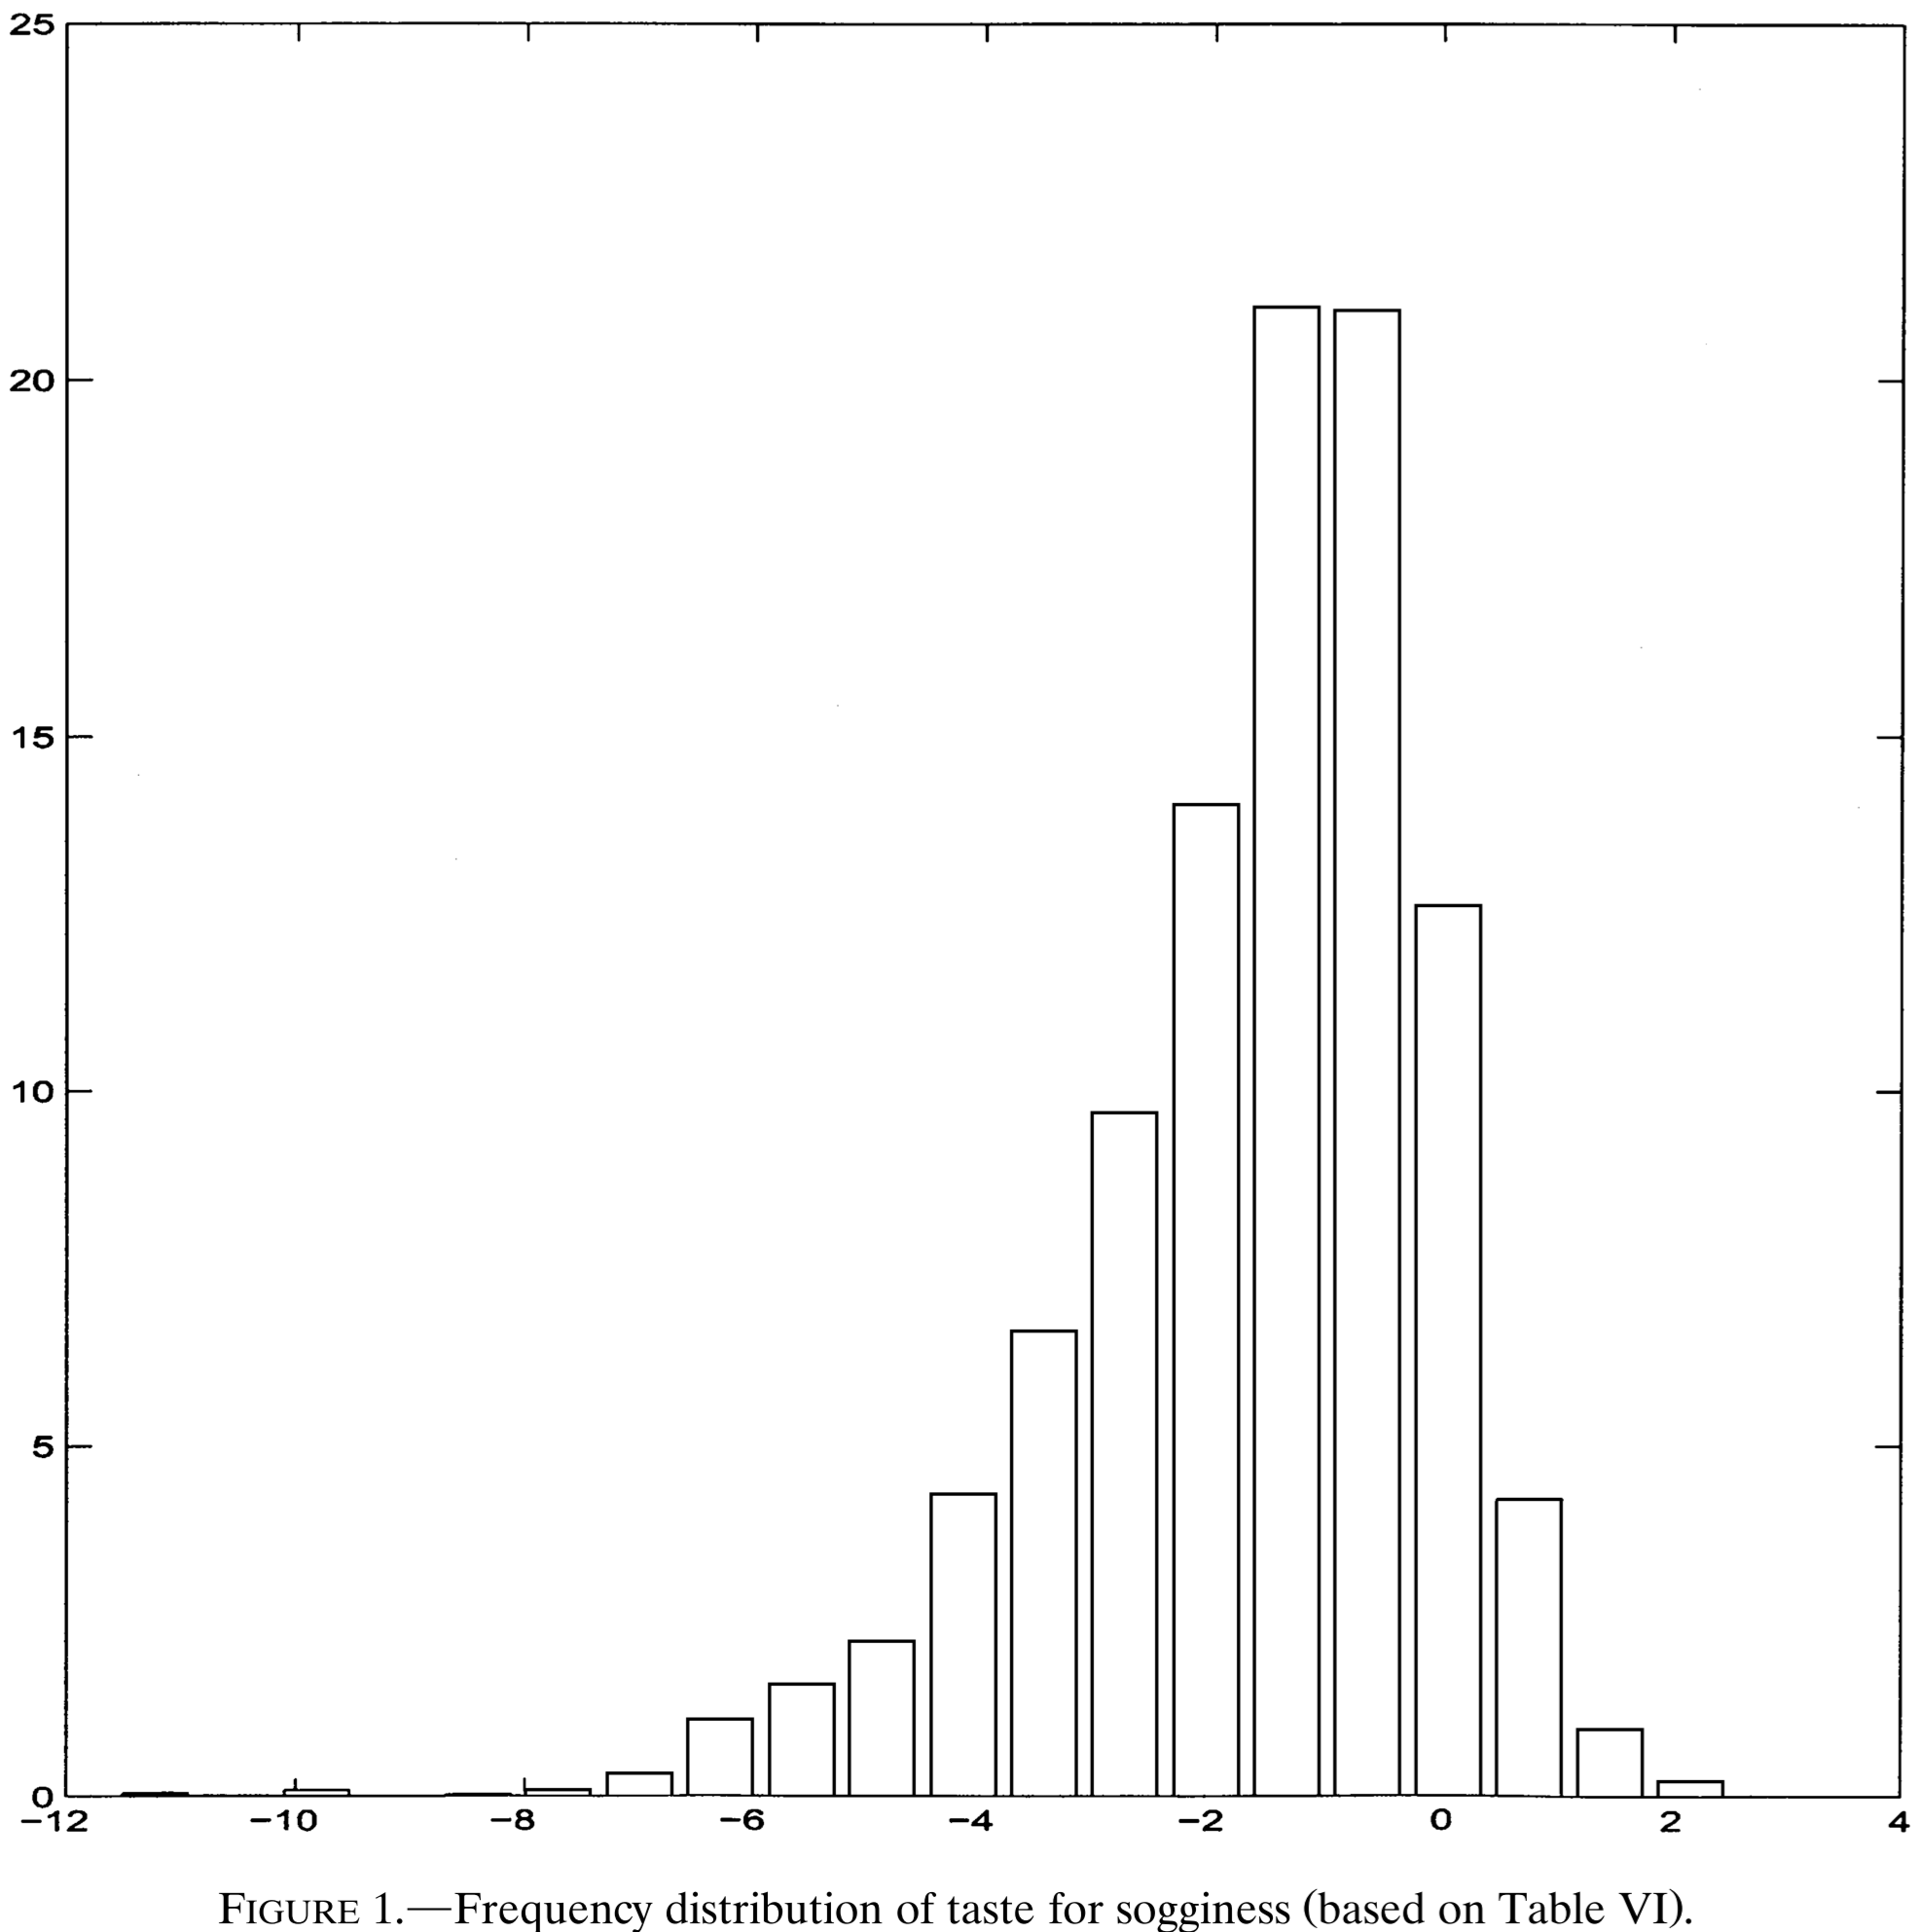
\includegraphics[scale=0.21]{figure1.png}
	\end{figure}
\end{frame}
%------------------------------------------------
\begin{frame}{Distribution of the Individual Price Sensitivity}
	\begin{figure}[h]
		\centering
		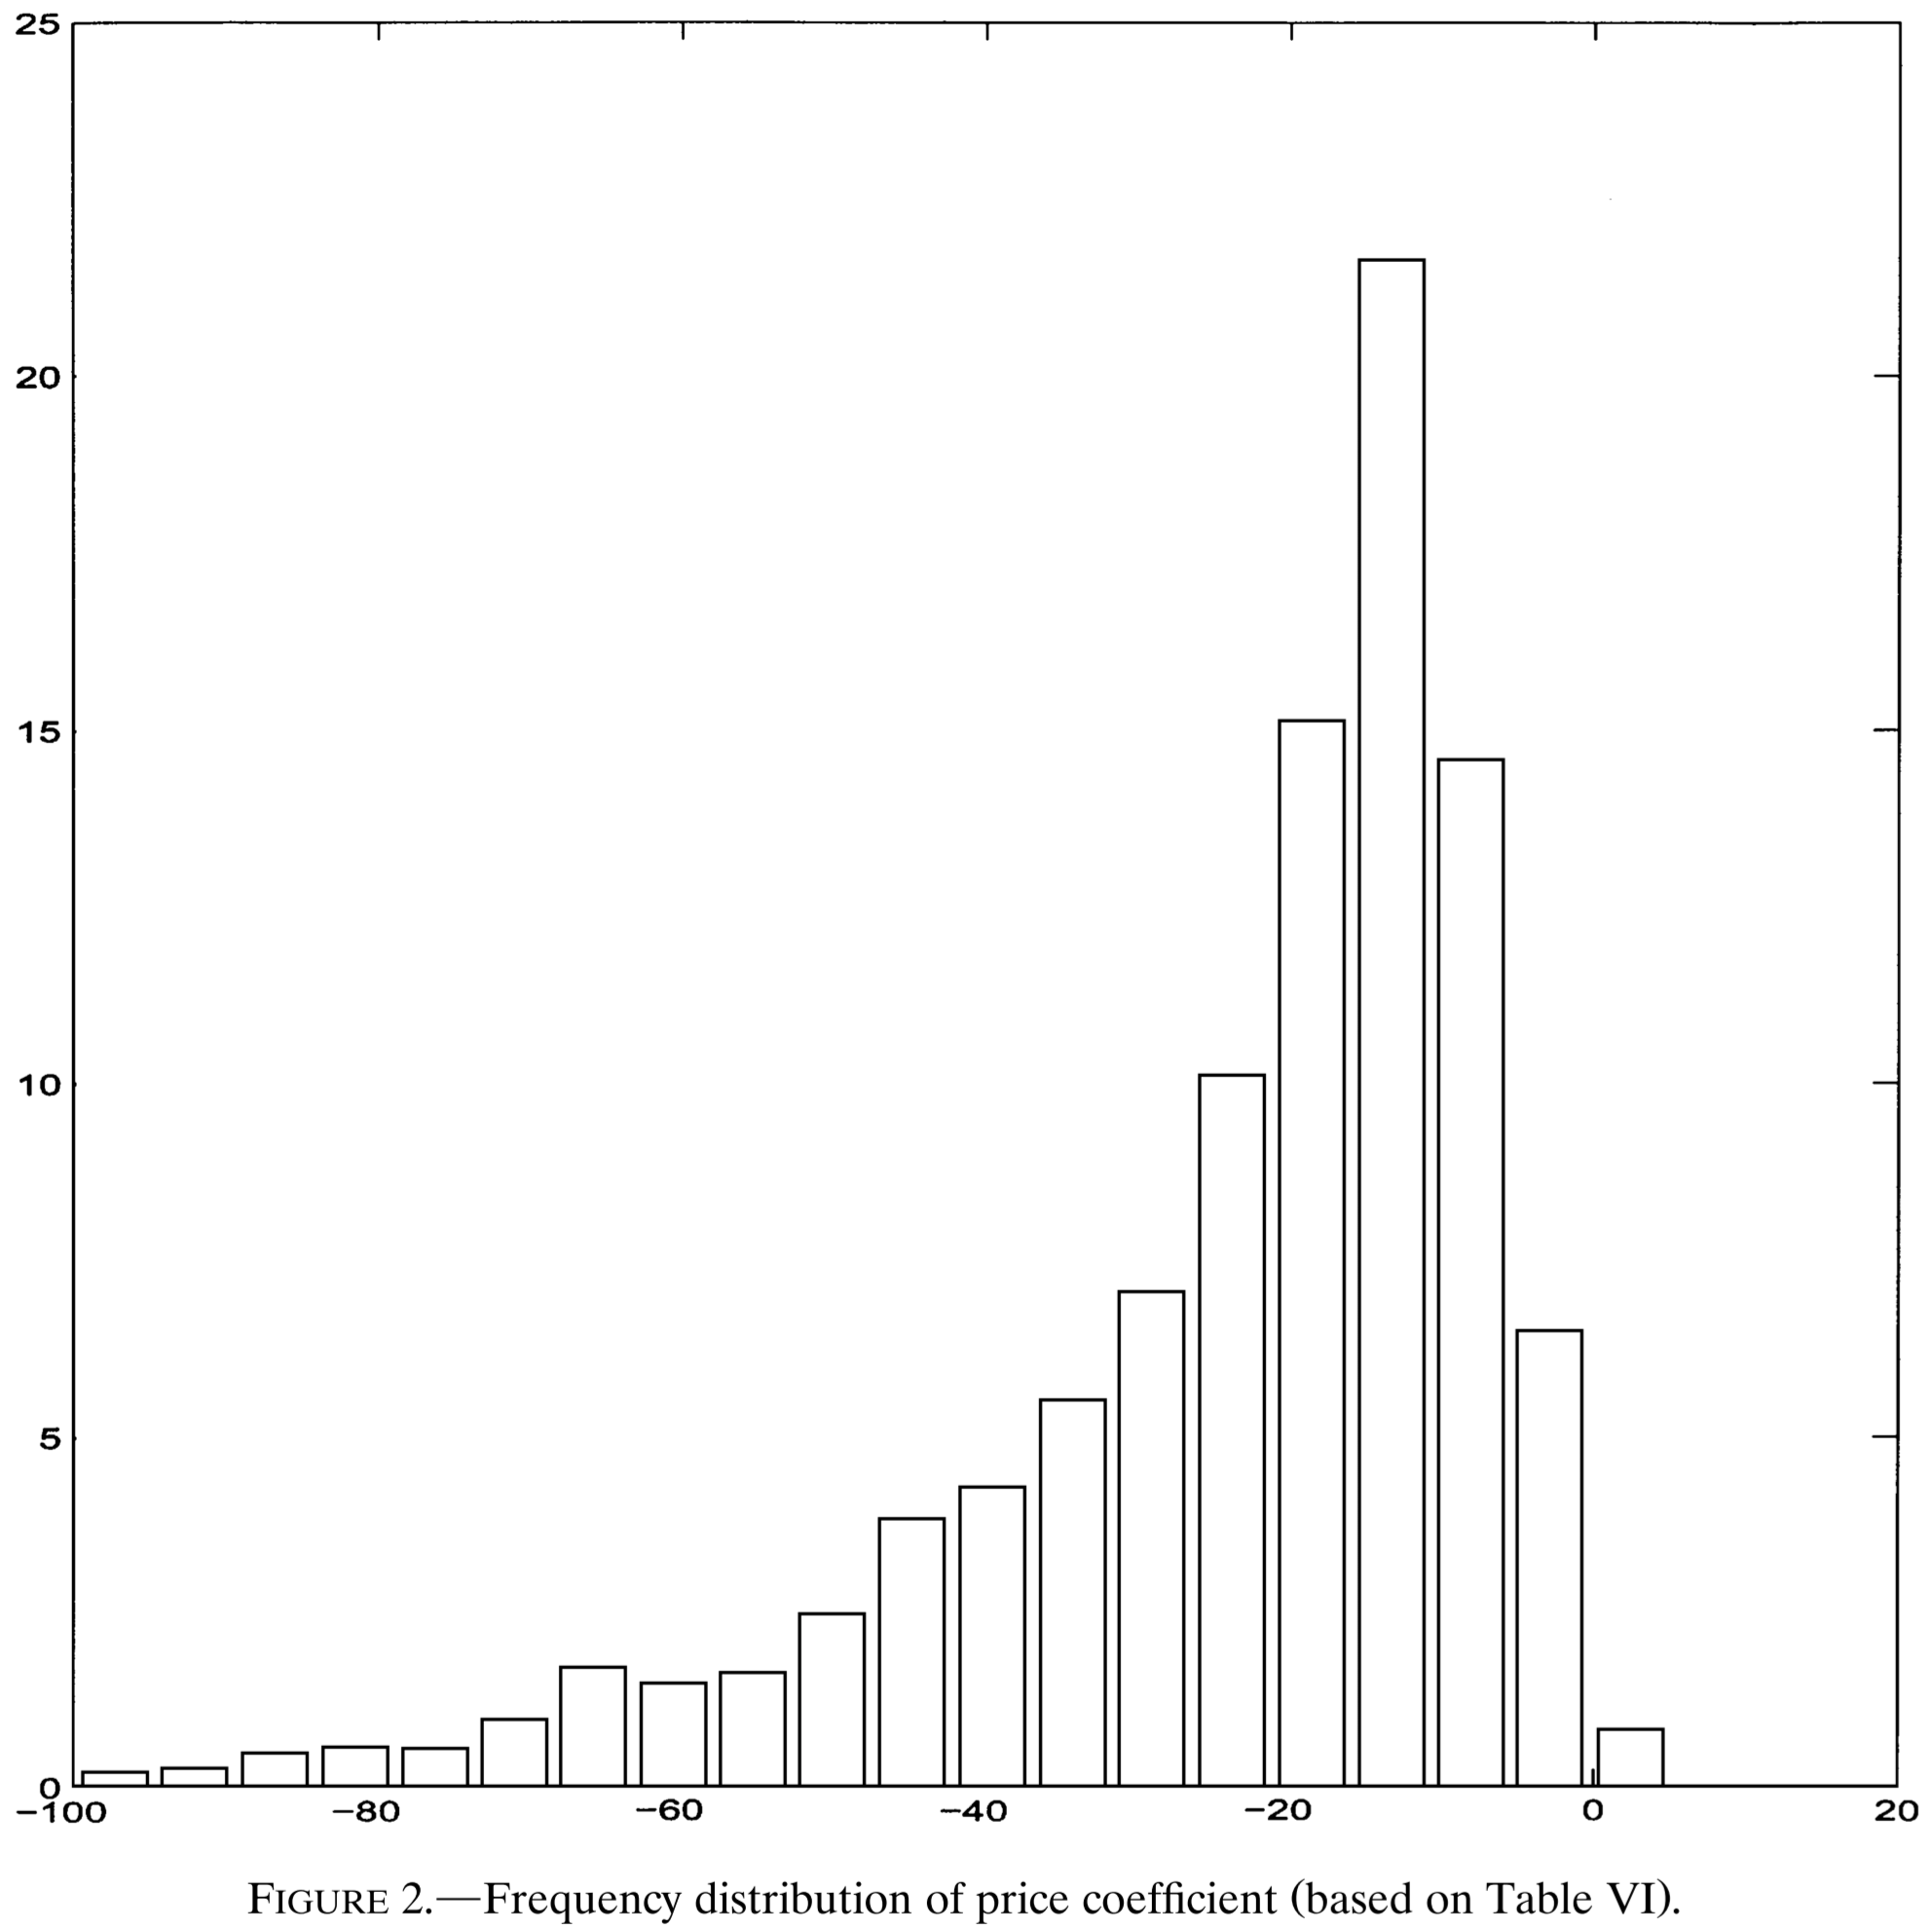
\includegraphics[scale=0.21]{figure2.png}
	\end{figure}
\end{frame}
%------------------------------------------------
\begin{frame}{Median Own and Cross-Price Elasticities}
	\centering
	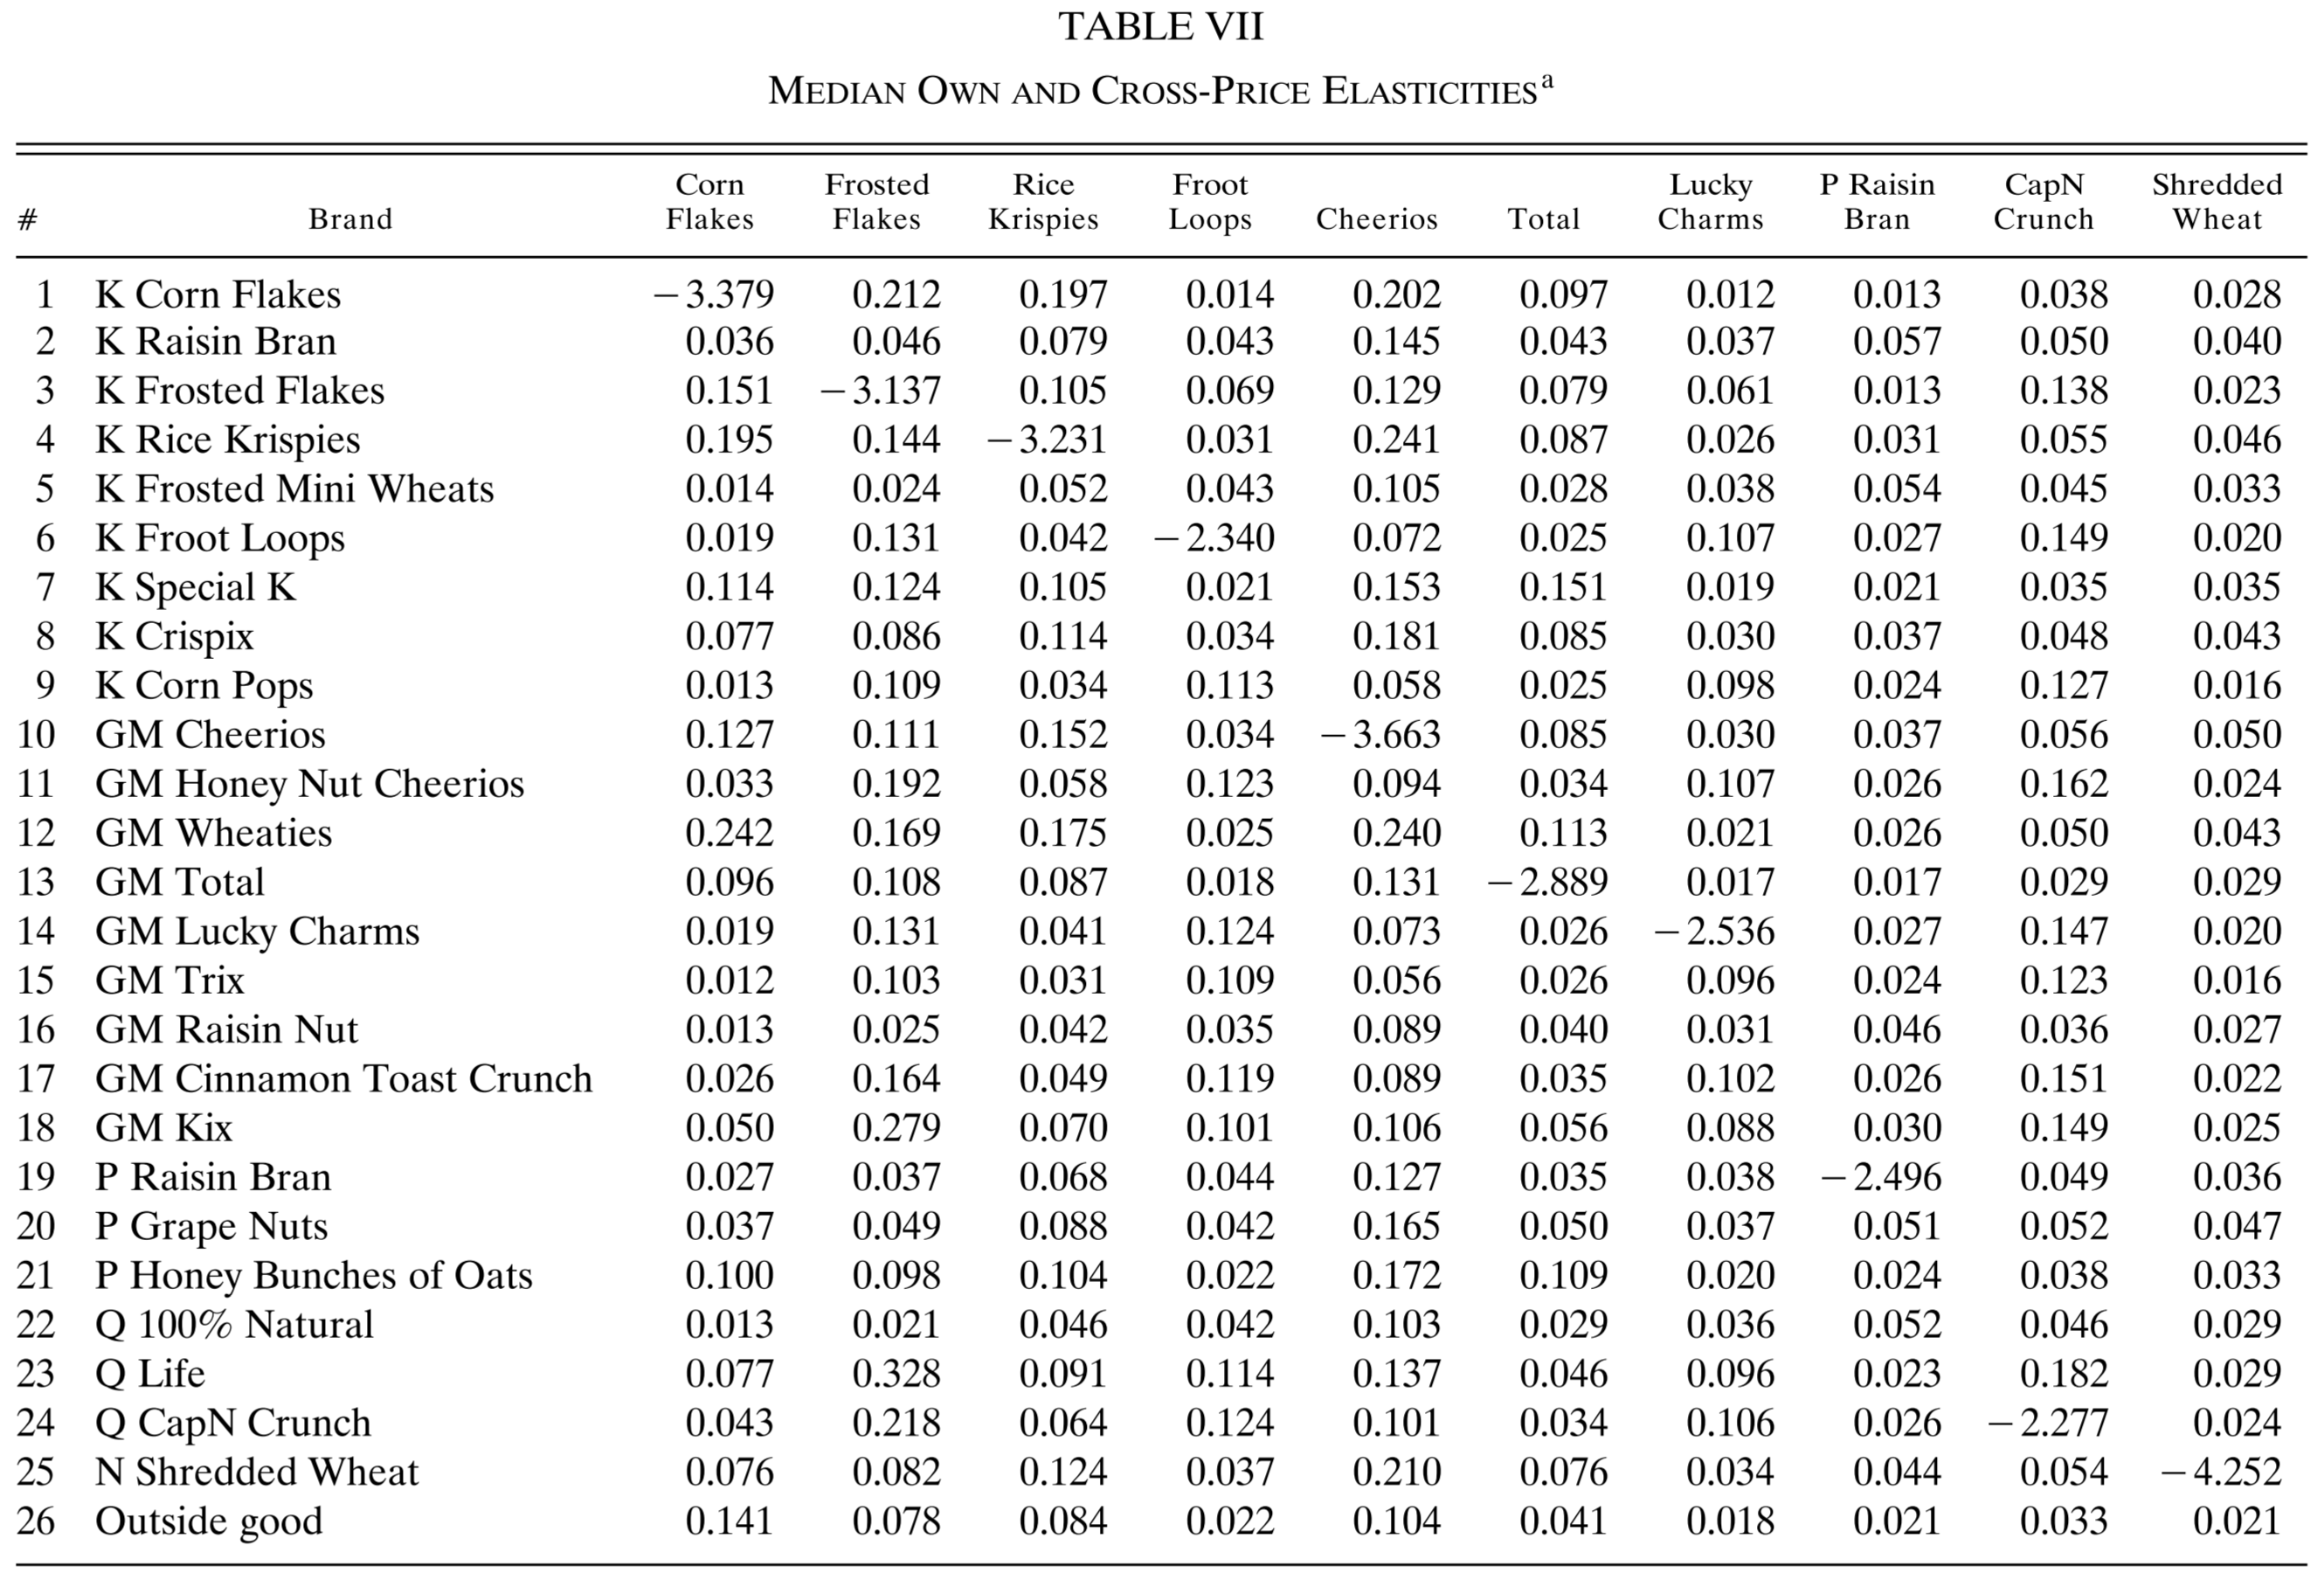
\includegraphics[scale=0.22]{table7.png}
\end{frame}
%------------------------------------------------
\begin{frame}[label=table8]{Price-Cost Margins}{Predicted PCM}
	\begin{itemize}
		\item compute PCM for three hypothetical industry structures
		\item Recall: $p-mc=\Omega^{-1}s(p)$.
	\end{itemize}

	\begin{figure}[h]
		\centering
		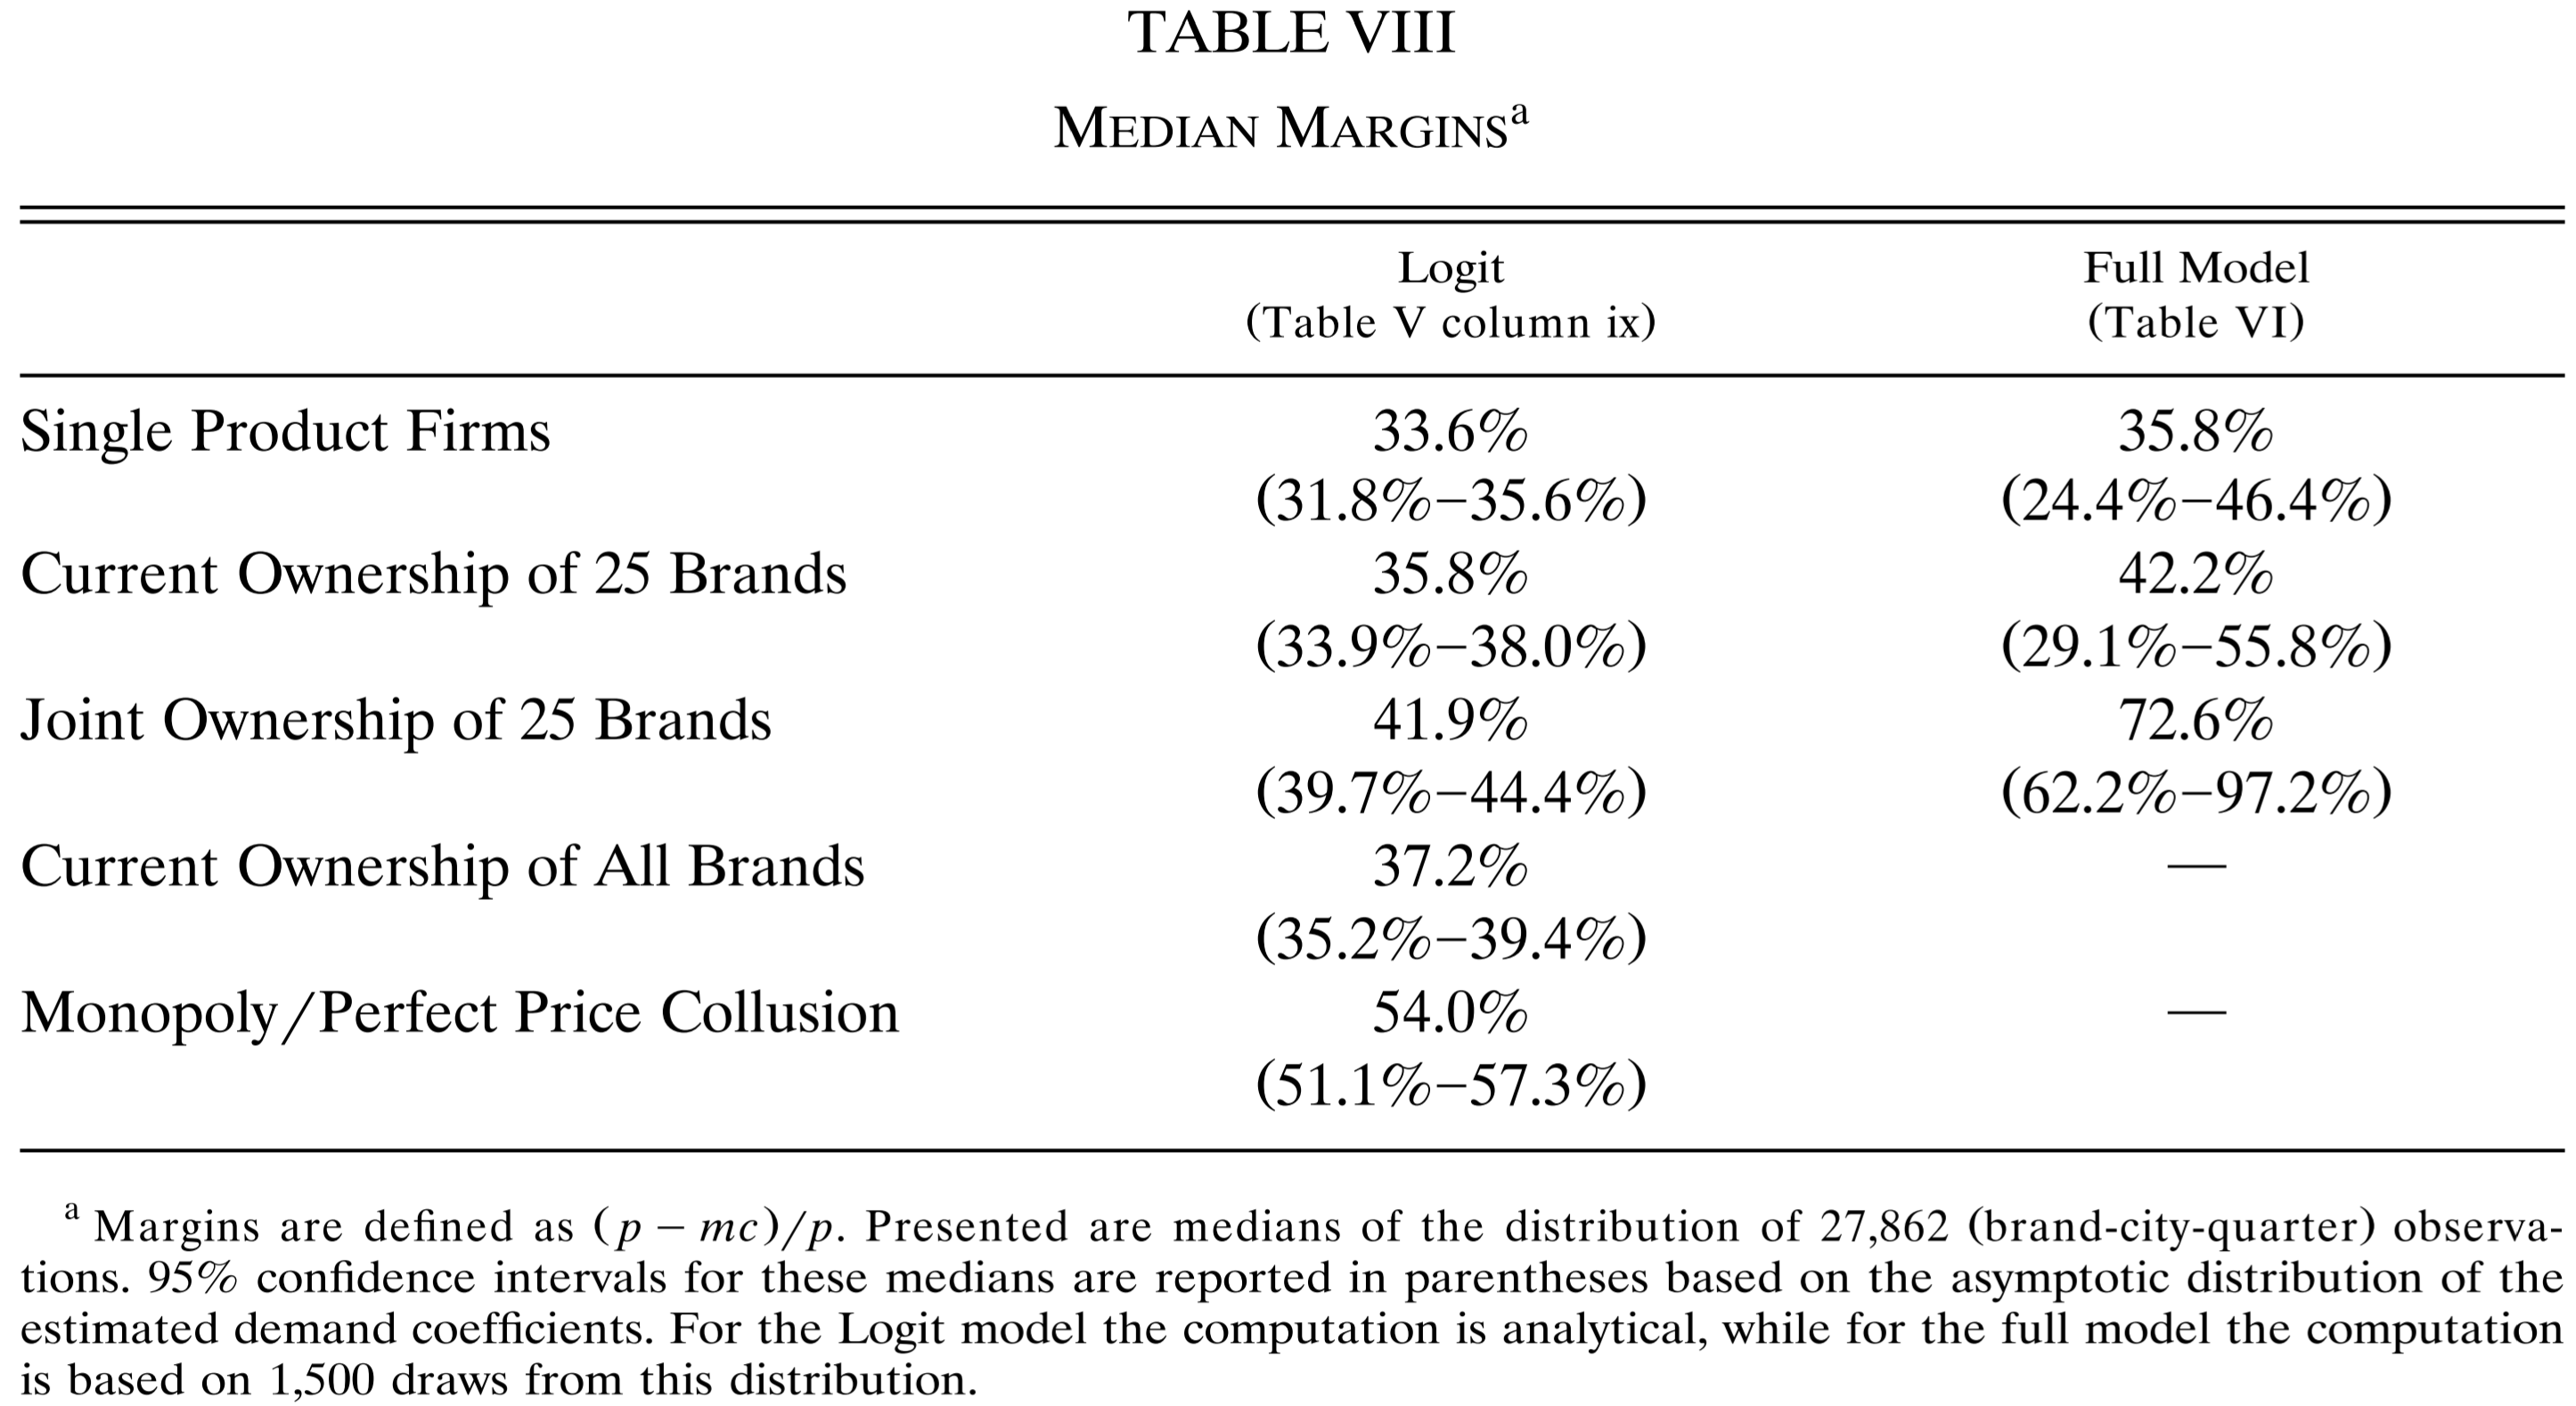
\includegraphics[scale=0.15]{table8.png}
	\end{figure}
	\hyperlink{logit}{\beamergotobutton{Back to Table 5}}
\end{frame}
%------------------------------------------------
\begin{frame}{Price-Cost Margins}{Observed PCM}
	\begin{figure}[h]
		\centering
		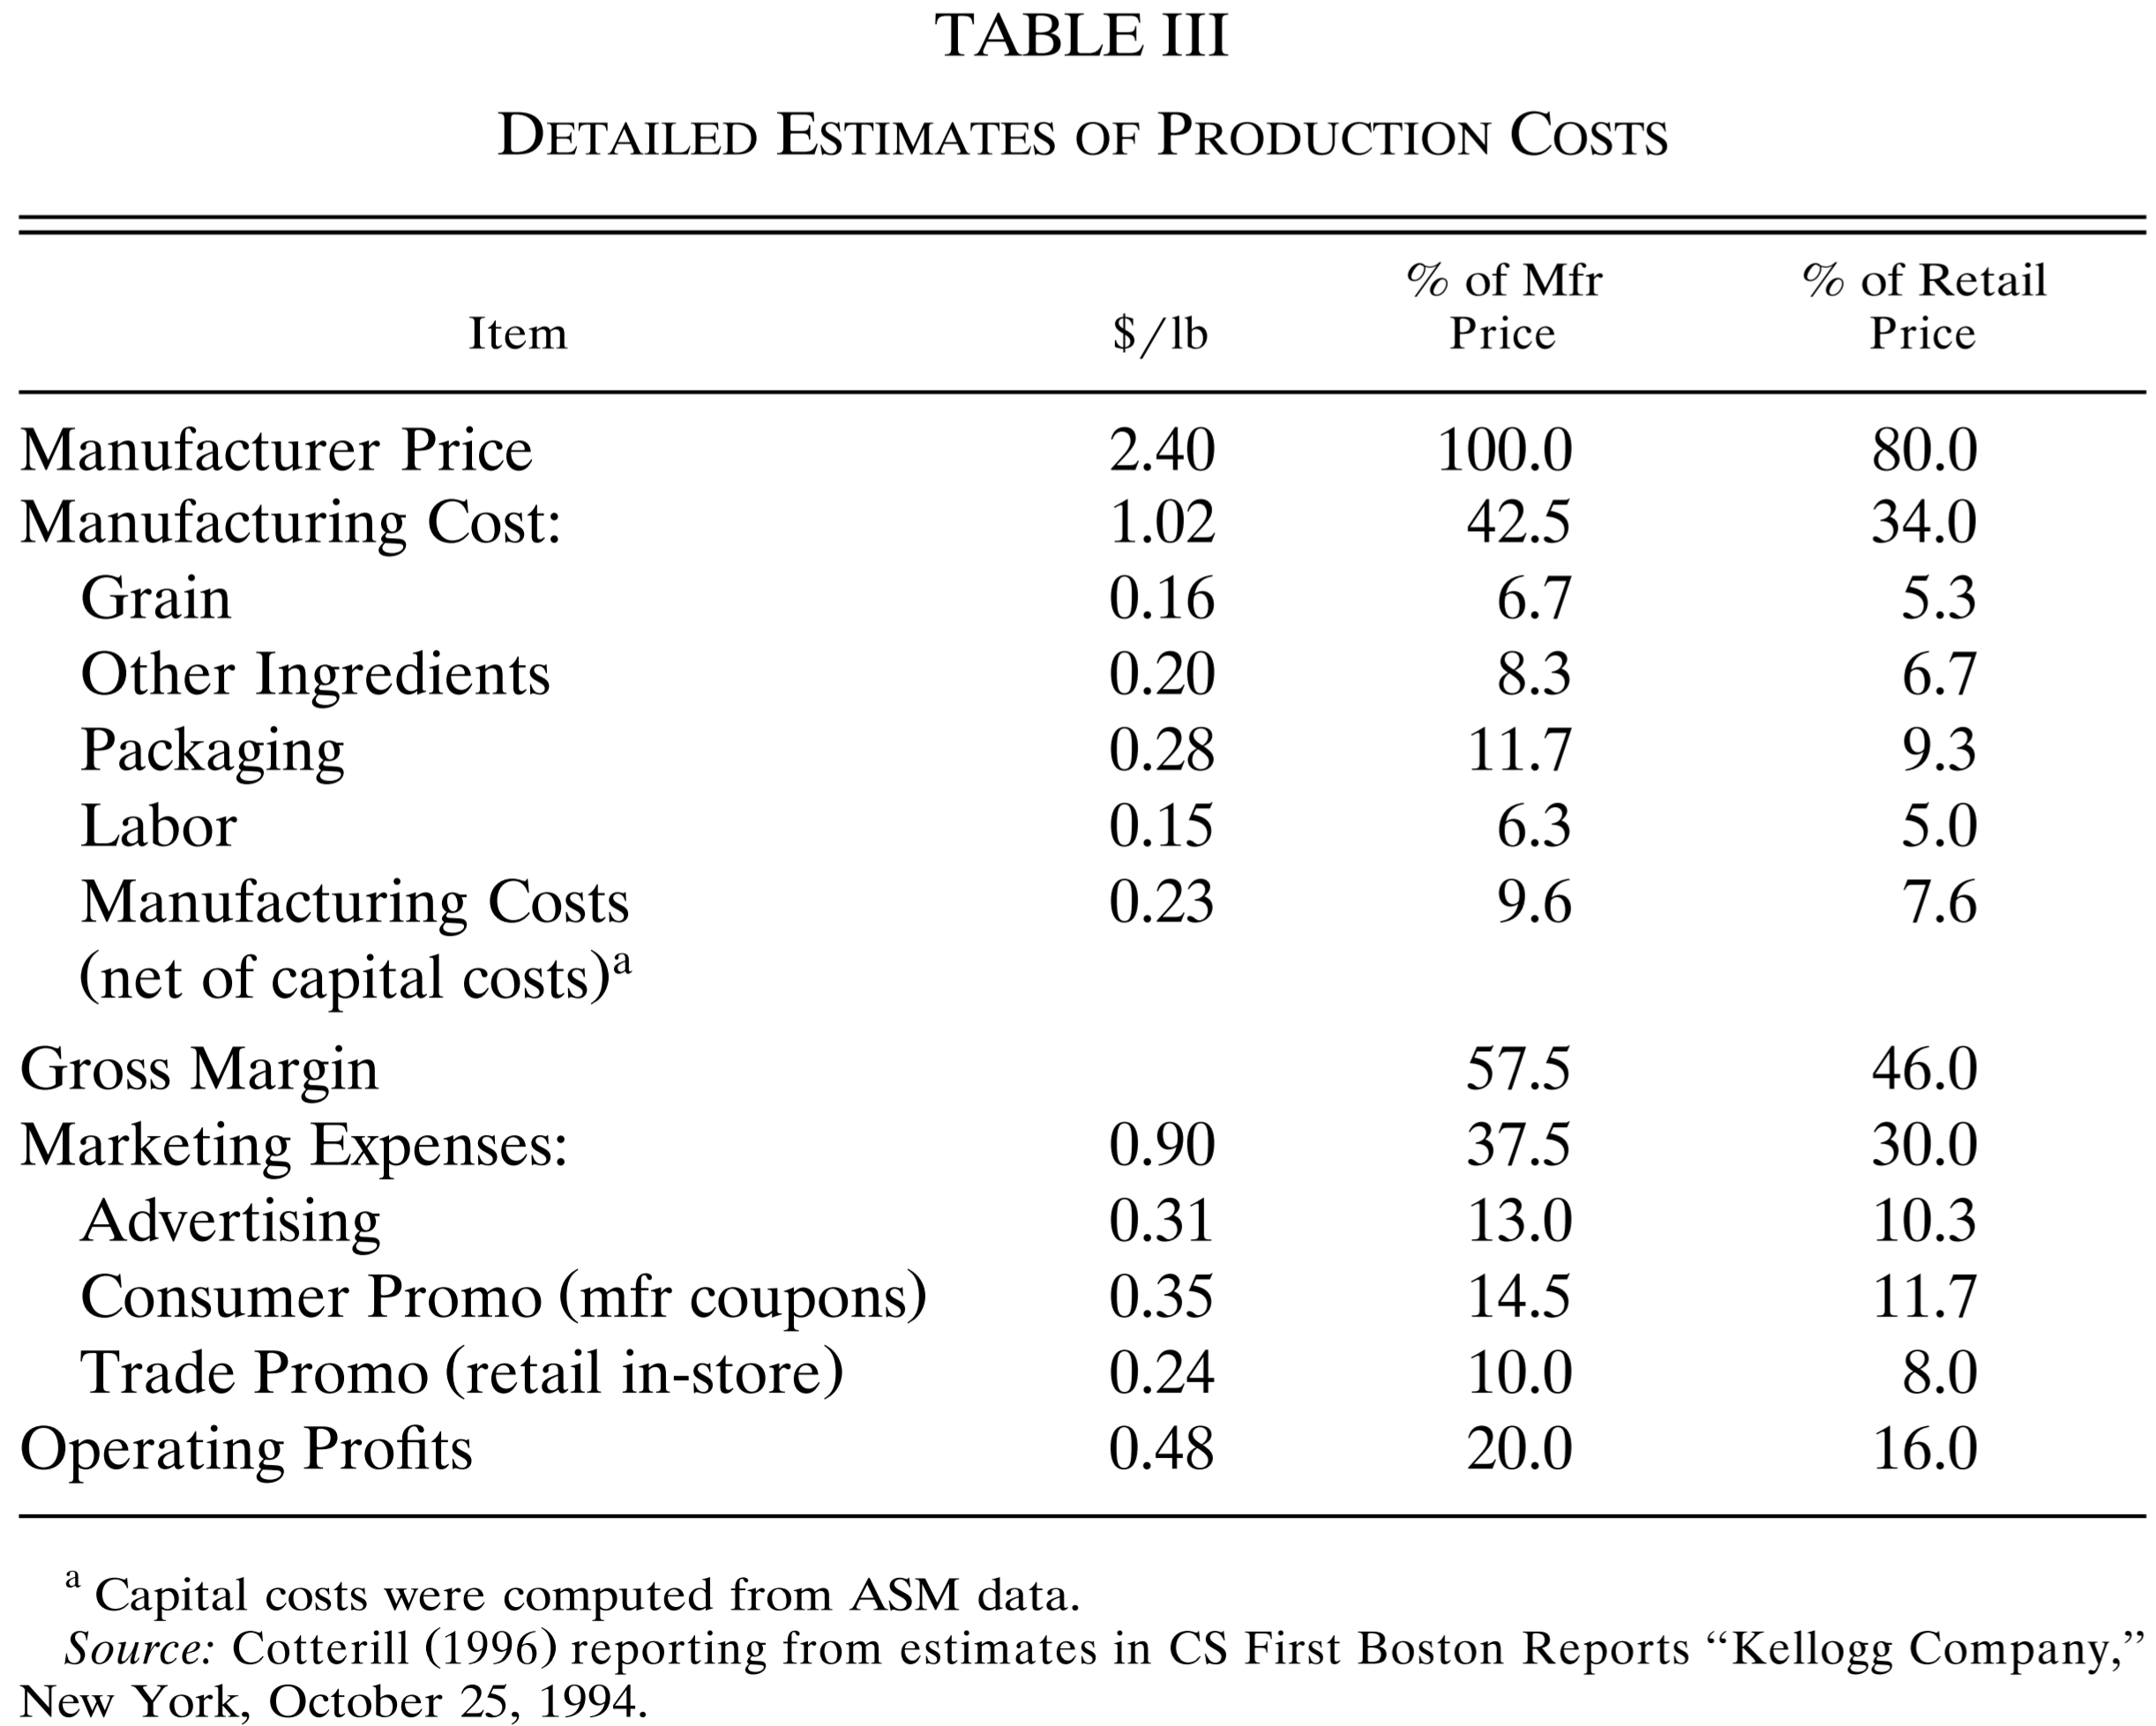
\includegraphics[scale=0.2]{table3.png}
	\end{figure}
\end{frame}
%------------------------------------------------

\section{Conclusions and Extensions}
\begin{frame}
	\transfade
	\tableofcontents[sectionstyle=show/shaded,subsectionstyle=show/shaded/hide]
	\addtocounter{framenumber}{-1}
\end{frame}
%------------------------------------------------
\begin{frame}{Conclusions}
	\begin{itemize}
		\item This paper uses a random coefficients discrete choice (mixed logit) model to estimate a brand-level demand system for RTE cereal.
		\item Parameter Identification exploits the panel structure of the data, and is based on an independence assumption of demand shocks across cities for each brand.
		\item If we are willing to accept Nash-Bertrand as a benchmark of noncollusivepricing, we are left to conclude, unlike previous work, that even with PCM greater than 45\%, prices in the industry are not a result of collusive behavior.
	\end{itemize}
\end{frame}
%------------------------------------------------

%--------------

%------------------------------------------------

\begin{frame}
\Huge{\centerline{\textit{The End}}}
\end{frame}
%----------------------------------------------------------------------------------------


\end{document} 